\renewcommand{\chaptername}{Chapter} 
\chapter{Limitations and Challenges in Methodology}\label{chap5}

In our study presented in Chapter \ref{chap4}, analyzing the representation + noise data allowed us to identify distinct pathological profiles and uncover the diverse sensory and cognitive mechanisms underlying prosody processing impairments after stroke. These two biomarkers hold significant potential for clinical applications, making their precise estimation crucial to ensure their reliability as long-term diagnostic tools. However, since not all patients exhibited deficits in both parameters, examining extreme cases can provide valuable insights into the potential neurological bases of these abnormalities. Yet, an important question remains: are these cases truly extreme, or do our estimation methods fail to accurately capture their impairments? We hypothesize that various factors could contribute to the uncertainty in these biomarkers, preventing them from being fully reliable.


\section {Number of trials}
In a reverse correlation experiment, one fundamental challenge is determining the sufficient number of trials required to obtain a robust estimation of both mental representation and internal noise.  Reverse correlation relies on stochastic stimuli sampling, meaning that more trials generally provide better statistical power. However, in a clinical population, practical constraints such as cognitive fatigue and attention span must also be considered when setting trial numbers.

\subsection{Number of trials as a challenge to stroke patients}
Stroke patients often experience post-stroke fatigue, which can significantly impact their ability to sustain attention during prolonged experimental sessions. This raises concerns about how many trials they can realistically complete without excessive cognitive strain affecting their performance. In our study, we limited the number of trials to 150, with an additional 50 double-pass trials for estimating internal noise.

One key question is whether this number of trials was already inducing fatigue in patients. To investigate this, we analyzed their reaction times across the 150 trials (see Figure \ref{fig:rt_clinical}). Our results did not reveal a consistent increase in reaction times (s), which would typically be expected if fatigue played a dominant role. Furthermore, when examining reaction times across three separate blocks of 50 trials each, we observed a noticeable decrease in reaction time (s) between the first and second blocks (see Figure \ref{fig:rt_block}).This pattern suggests two possible interpretations: Learning effect, ahe decline in reaction time may reflect improved task performance after initial exposure to the task structure and Loss of attention, alternatively, patients might have become less engaged in the task after the first block, leading to faster but potentially less controlled responses. Examining representation typicality, we observe that with increased learning, healthy participants show a progressive improvement in their mental representation across consecutive blocks (0.7 to 0.9). In contrast, stroke patients exhibit a decline, with their representation decreasing from block 1 to block 3 (0.65 to 0.45) (see Figure \ref{fig:kernel_typicality_block}).
\begin{figure}[H]
    \centering
    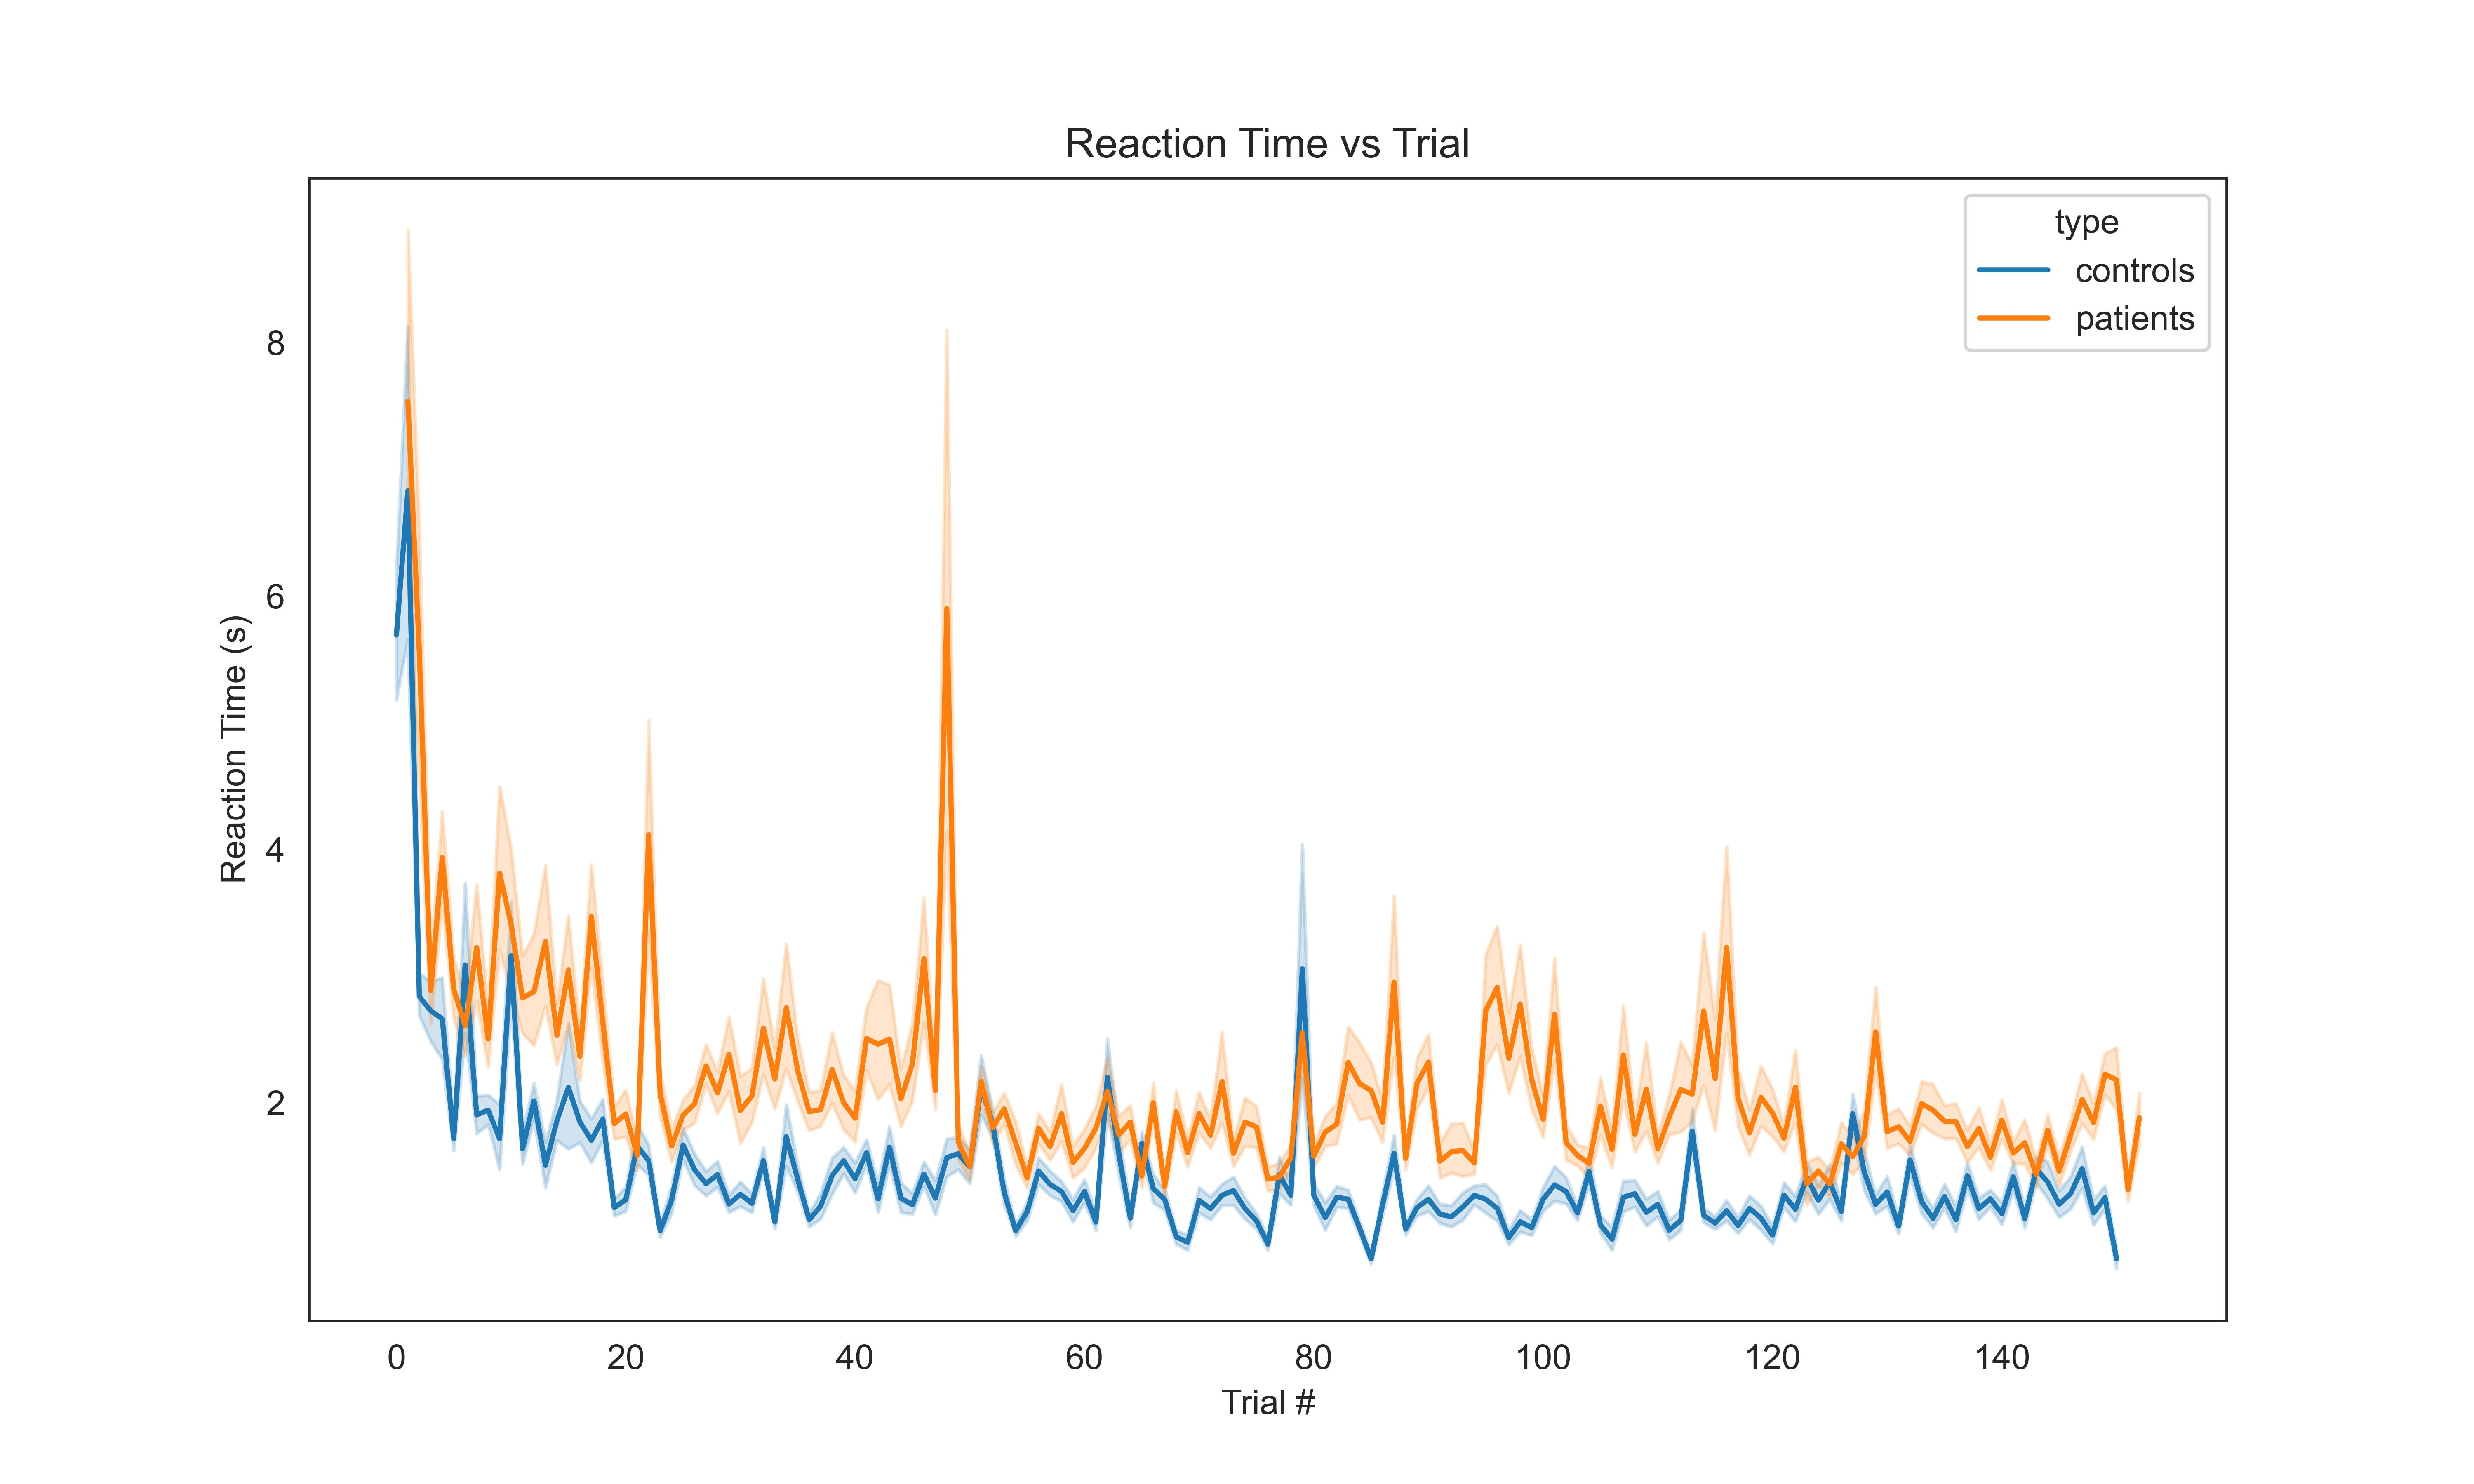
\includegraphics[width=15cm]{MainLayout/Images/chapter5/rt_clinical.jpg}
    \caption{Main Title for First Image \\ \small Subtitle for the first graphic.}
    \label{fig:rt_clinical}
\end{figure}

\begin{figure}[H]
    \centering
     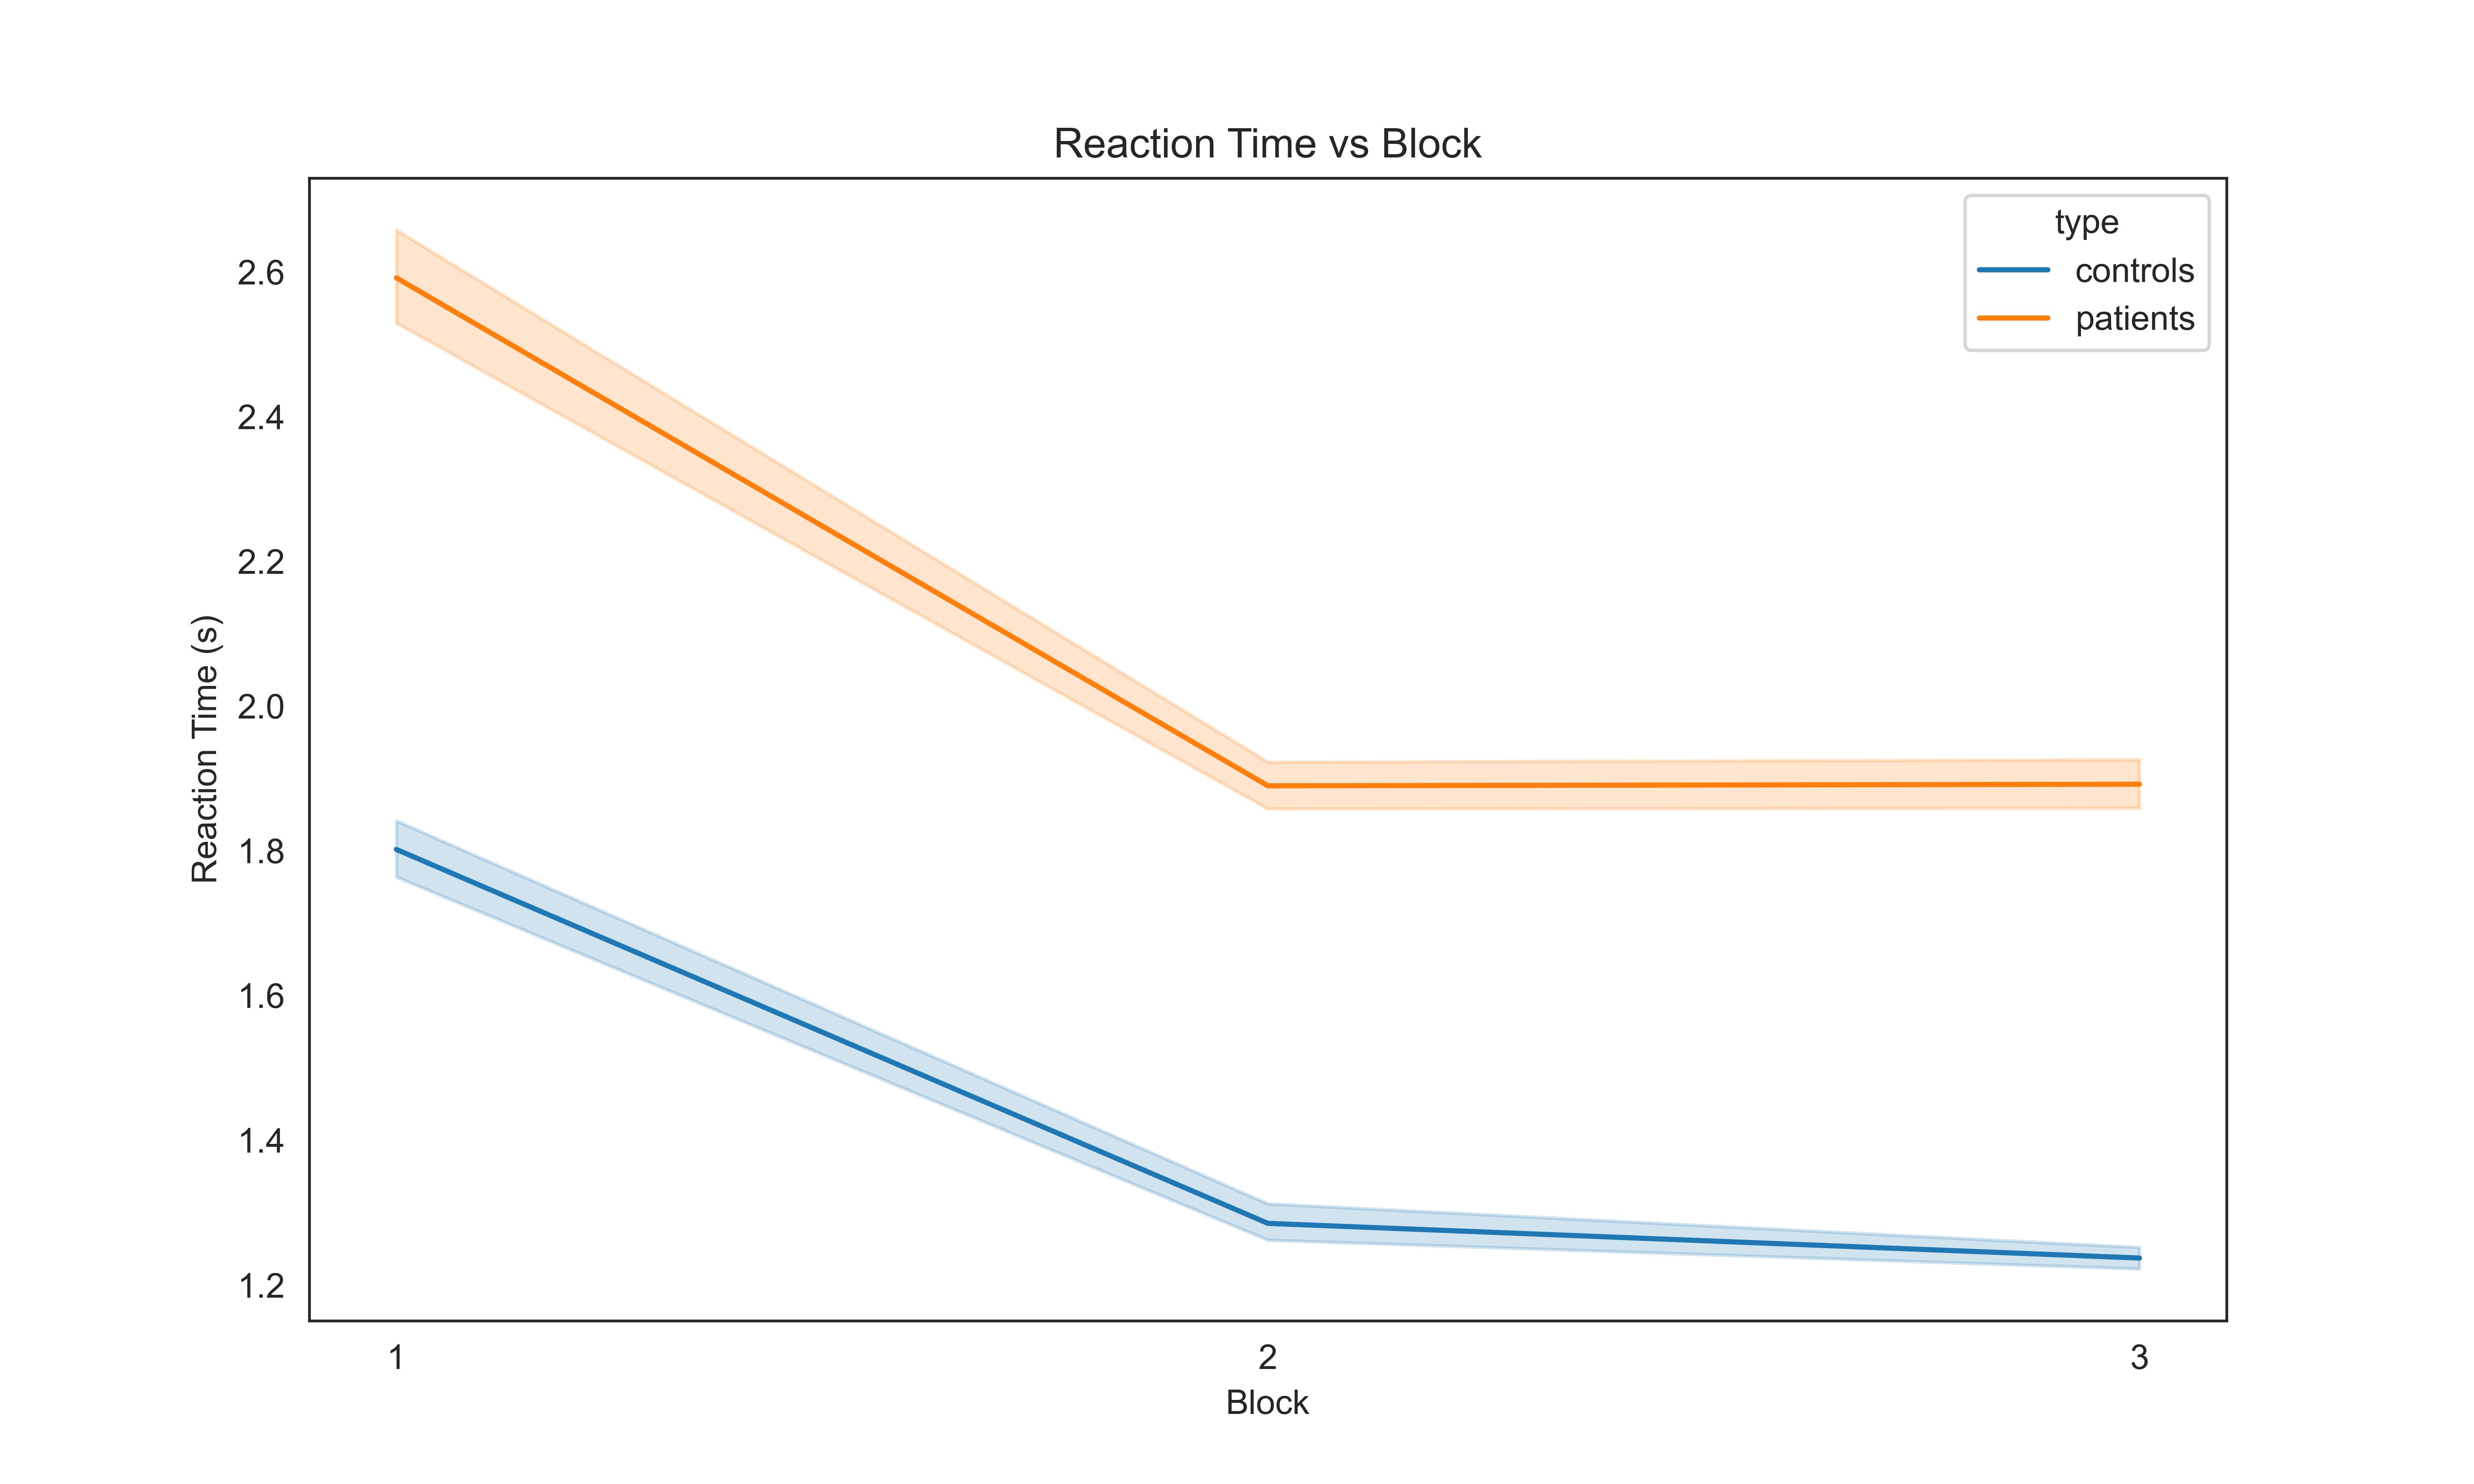
\includegraphics[width=15cm]{MainLayout/Images/chapter5/rt_block.jpg}
    \caption{Main Title for First Image \\ \small Subtitle for the first graphic.}
    \label{fig:rt_block}
\end{figure}

\begin{figure}[H]
    \centering
    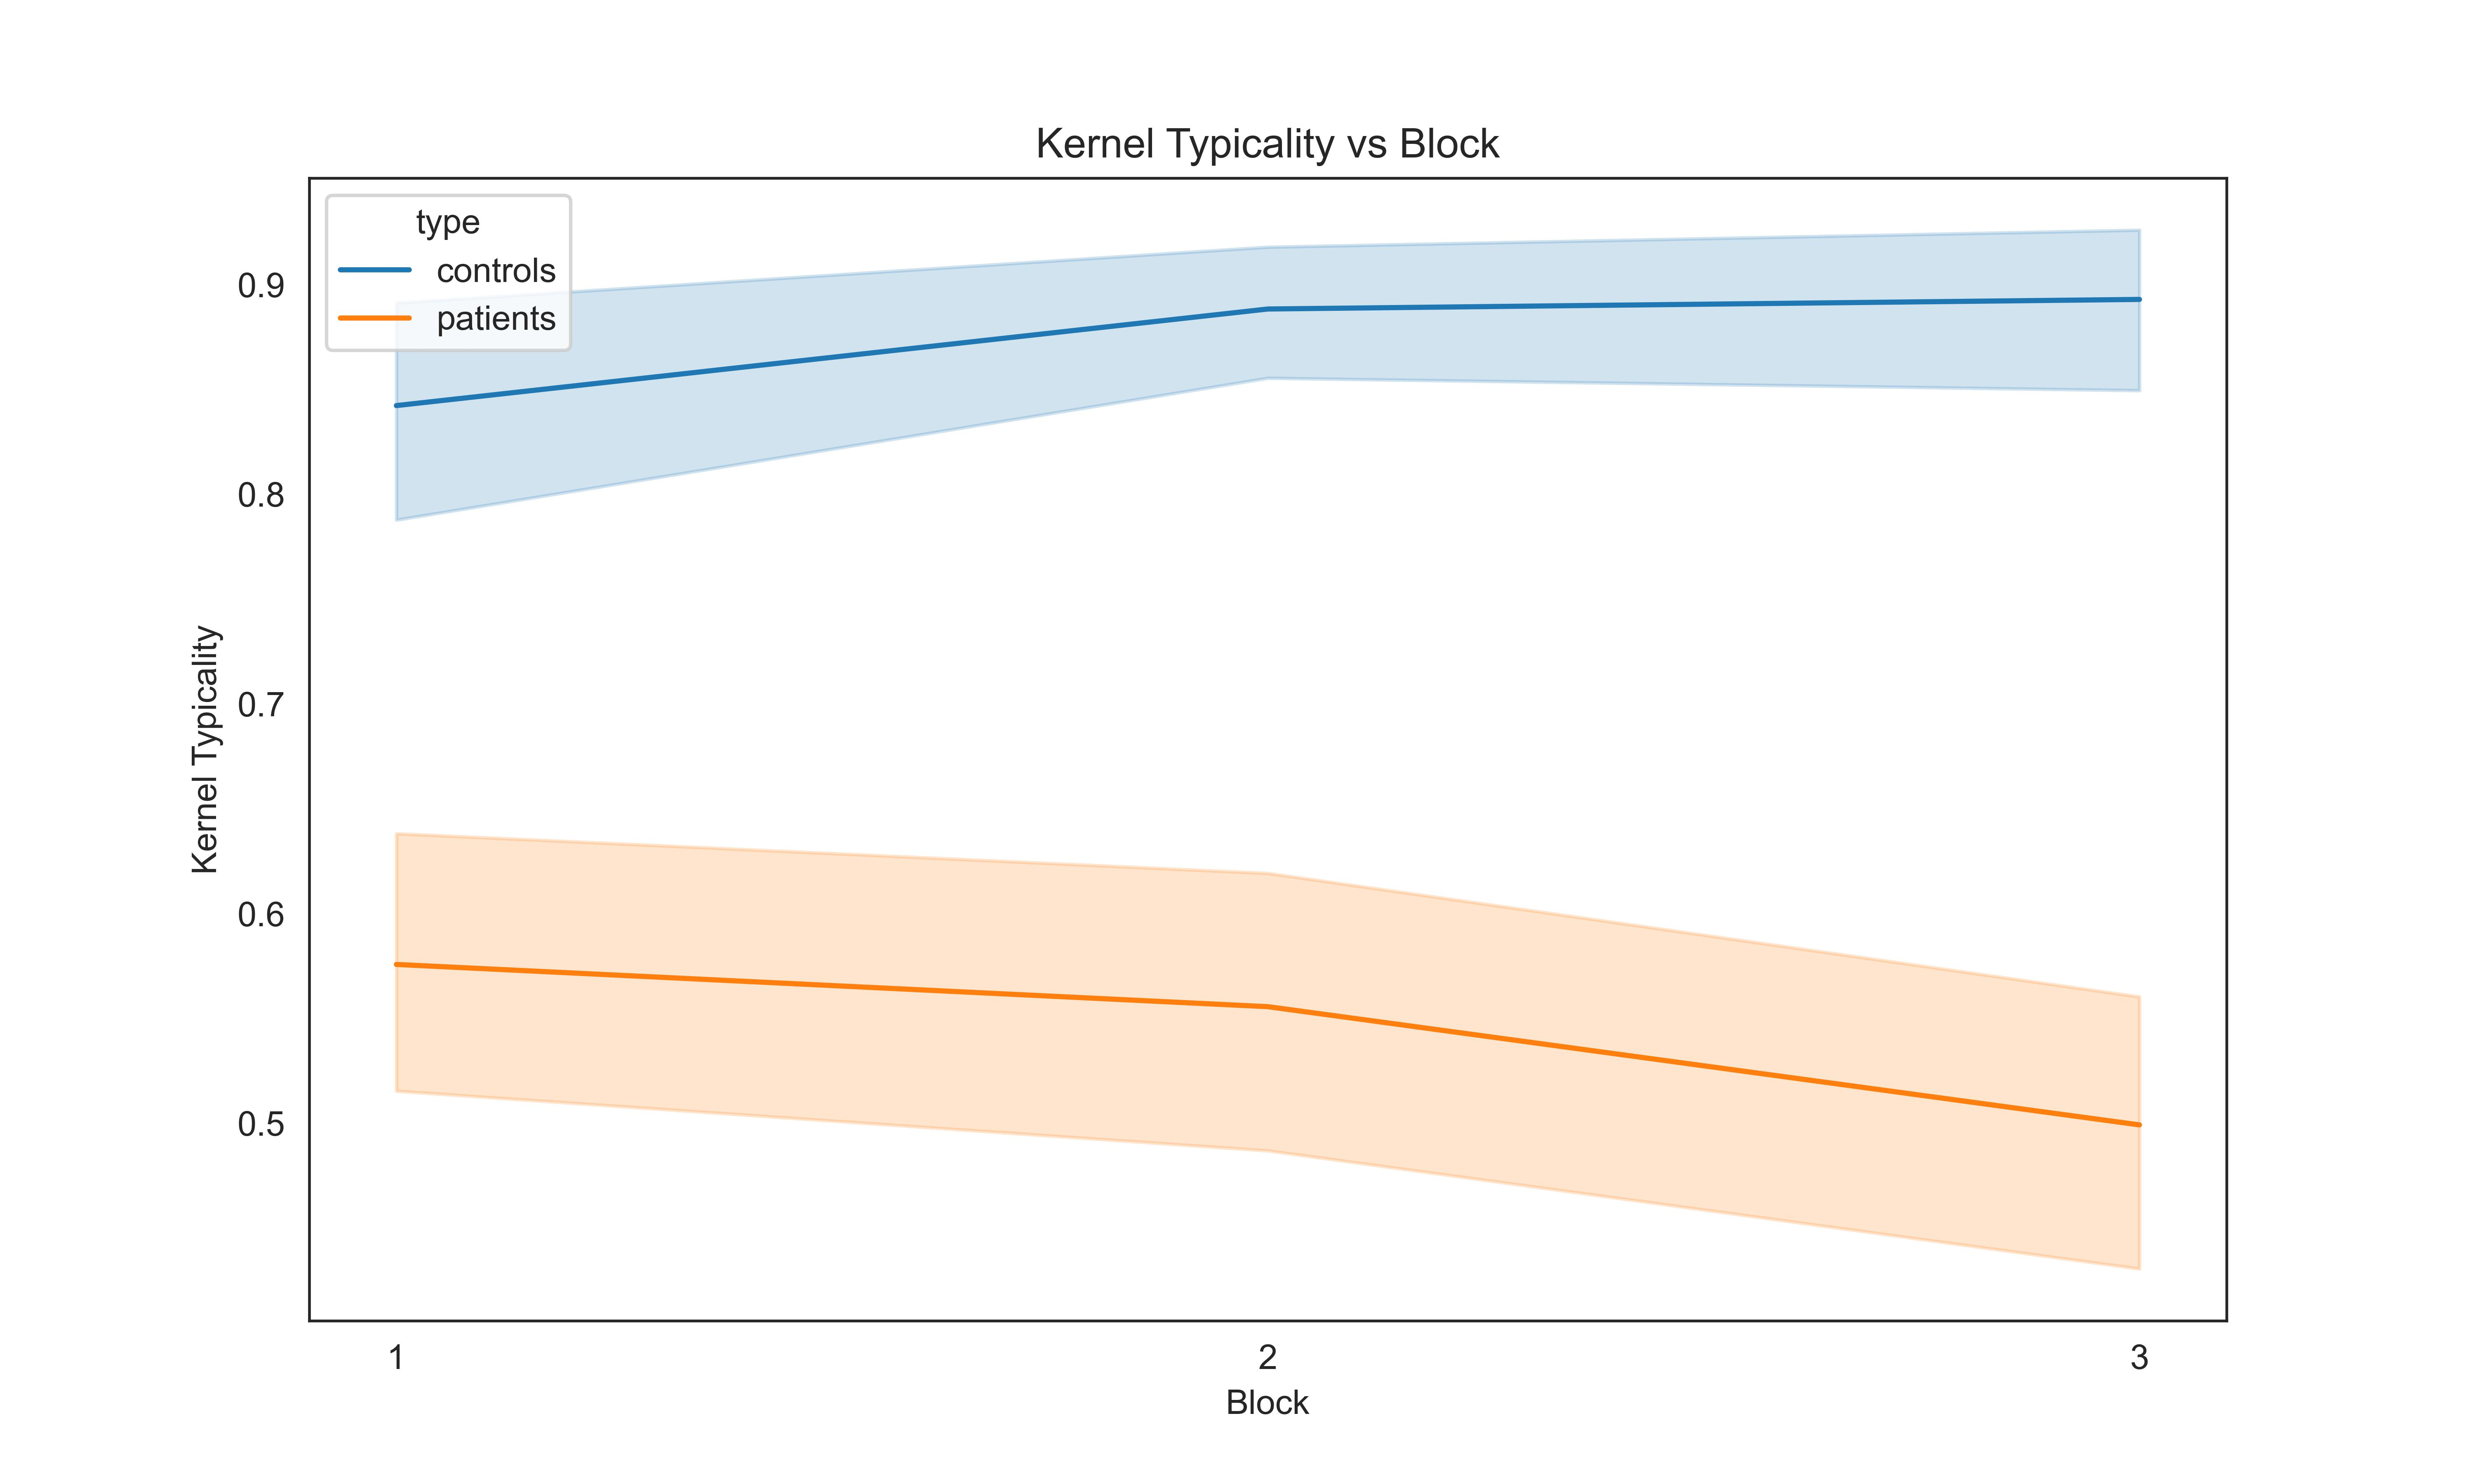
\includegraphics[width=15cm]{MainLayout/Images/chapter5/kernel_typicality_block.jpg}
    \caption{Main Title for First Image \\ \small Subtitle for the first graphic.}
    \label{fig:kernel_typicality_block}
\end{figure}

\subsection{Number of trials effects on kernel estimation}
TThe PALIN framework enables the simulation of a linear observer performing the same reverse correlation experiment as real participants but under controlled conditions. In this study, we simulate an experiment with a limited number of trials (n=150), as shown in Figure \ref{fig:kernel_150}. The observer is assigned a known true kernel and completes 50 double-pass trials. This simulation is repeated 1000 times to estimate the mental representation using two methods introduced in Chapter \ref{chap3}: the weighted sum kernel (blue) and the GLM kernel (orange). The estimation error (y-axis) is evaluated by calculating the correlation between the true kernel and the estimated kernel at different levels of true internal noise (x-axis). The shaded areas represent the variability (confidence intervals) across the 1000 simulations.
The vertical dashed lines in the figure highlight the mean internal noise levels for the two groups in the study, controls (blue, mean internal noise= 0.8) exhibit lower internal noise, corresponding to high kernel correlation (>0.95) and stroke atients (red, mean internal noise=2.8) tend to have higher internal noise, leading to reduced kernel correlation (approximately 0.85). Both kernel types demonstrate high kernel correlation at lower internal noise levels, but a progressive decline is observed as internal noise increases. In general, the limited number of trials (n=150) constrains the precision of kernel estimation, especially at higher noise levels. This limitation is evident in the divergence of the shaded regions, which reflects greater variability in estimation as internal noise increases.


\begin{figure}[H]
    \centering
    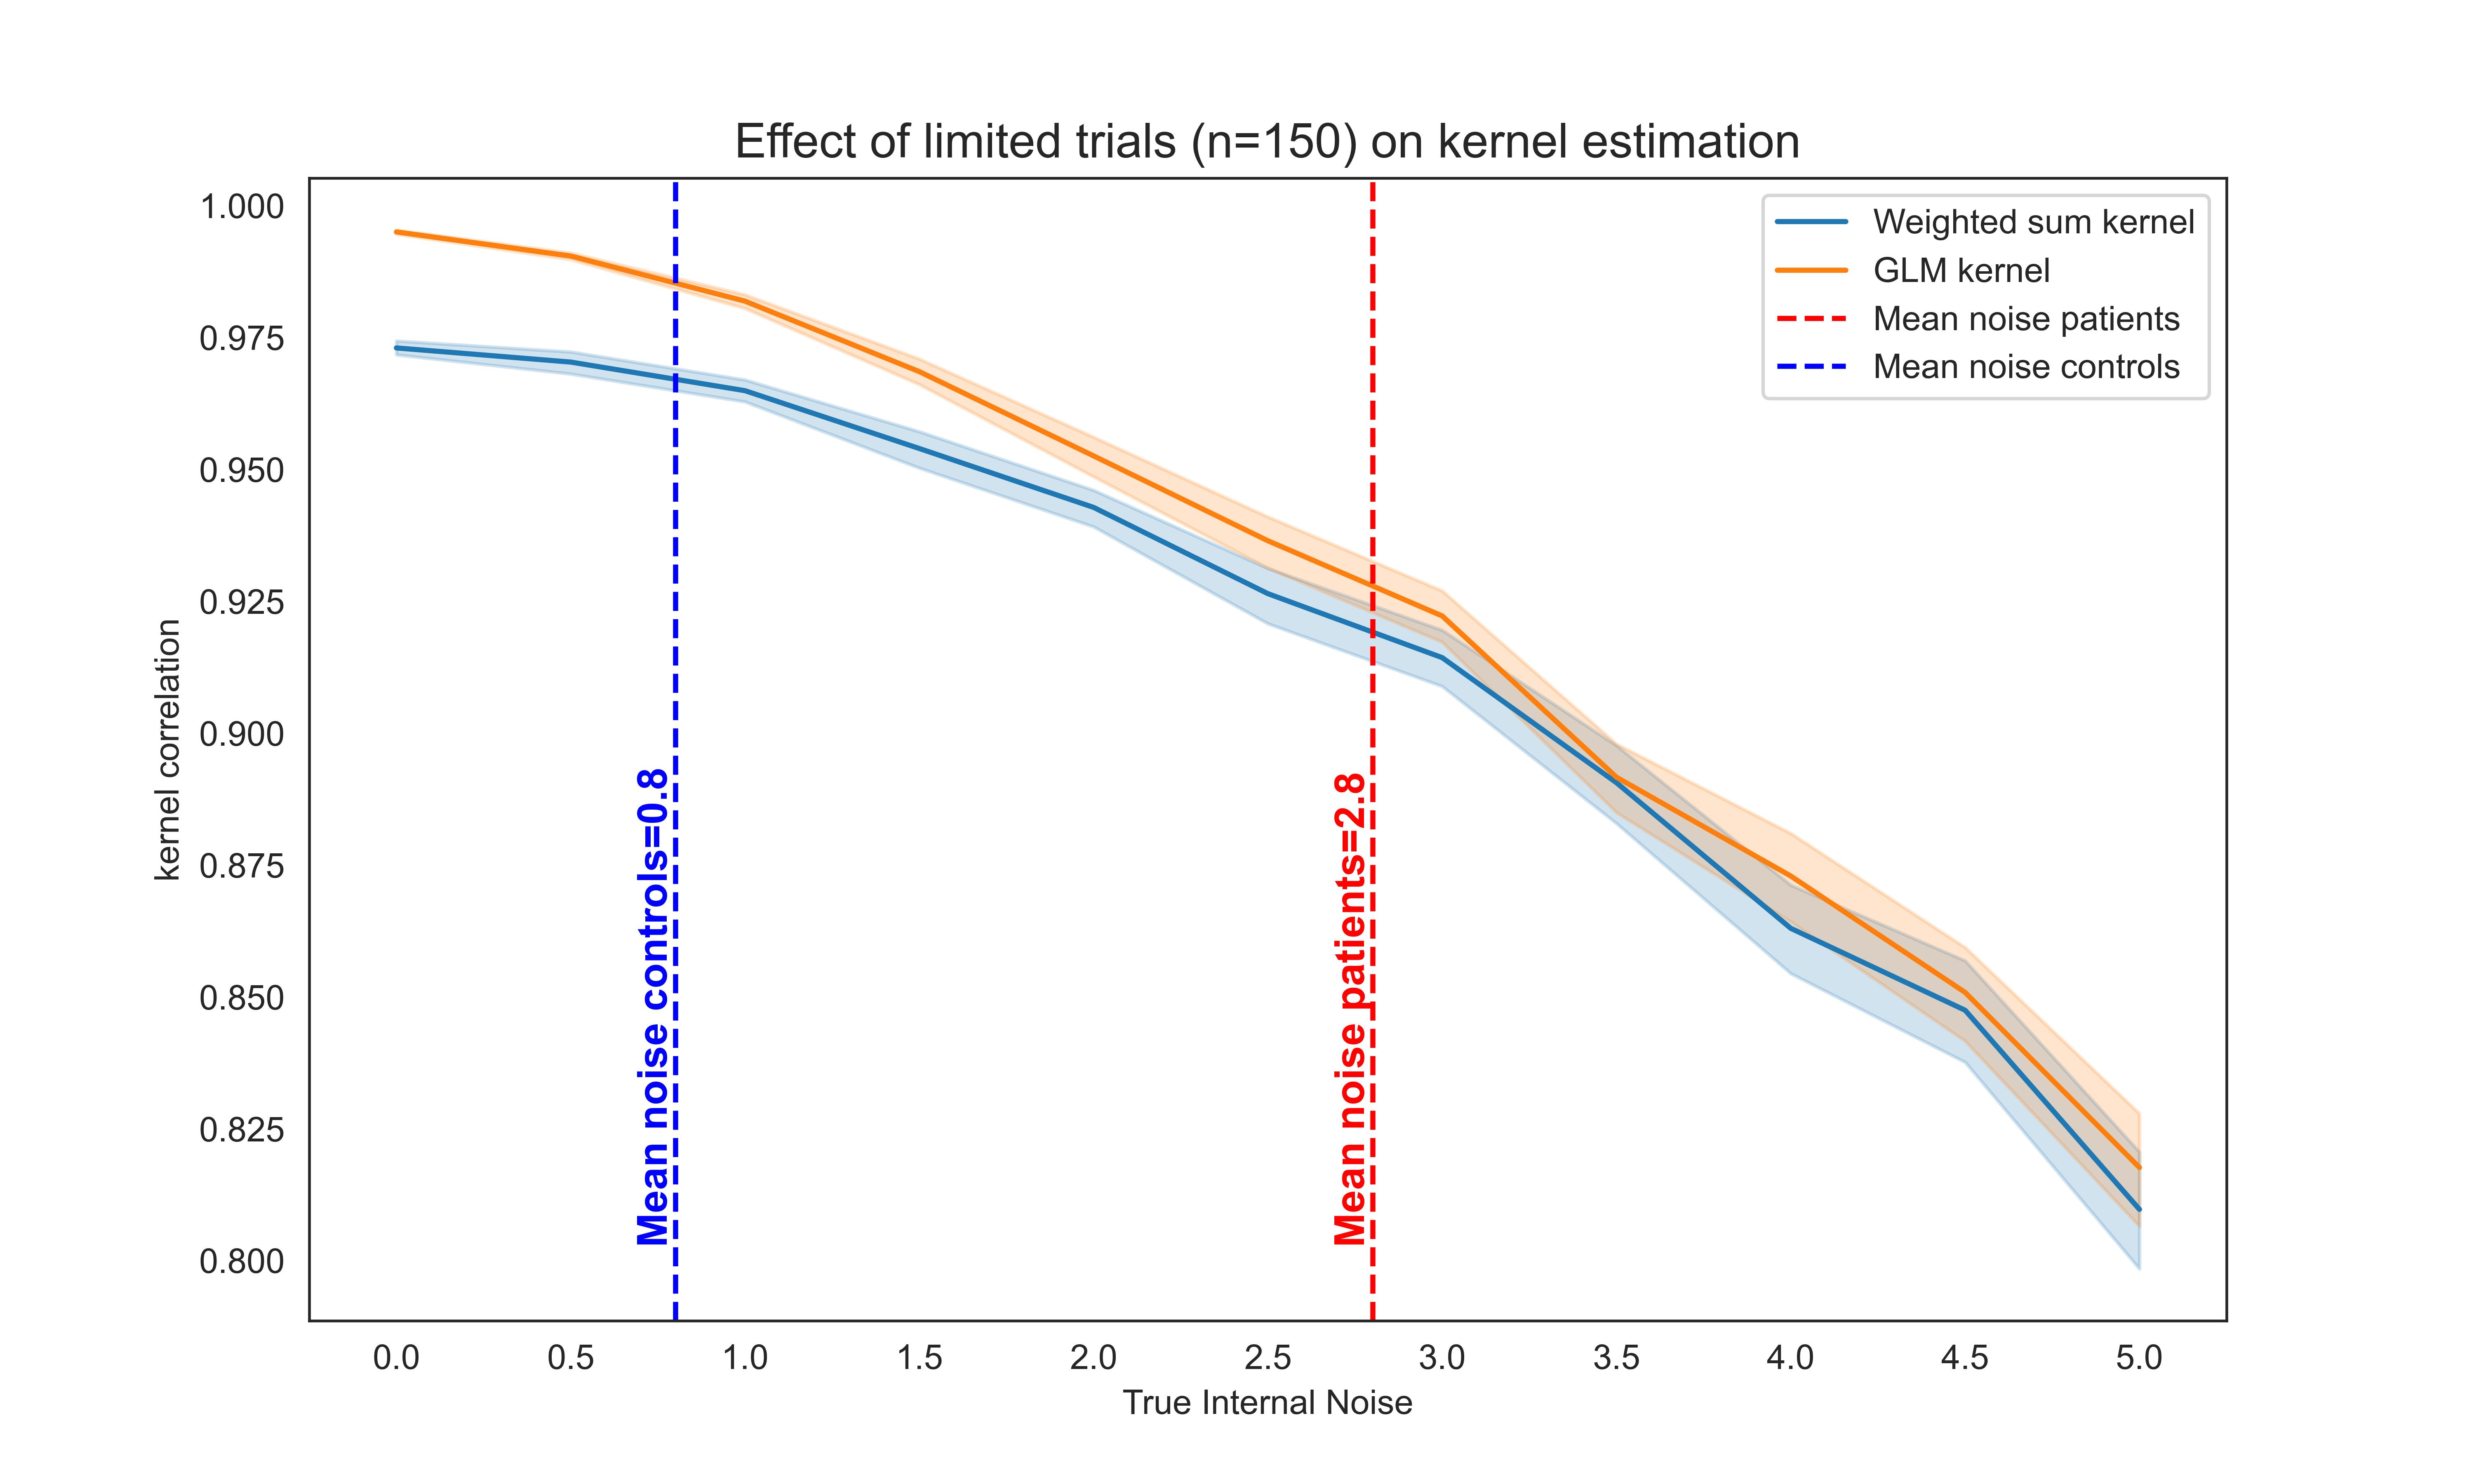
\includegraphics[width=15cm]{MainLayout/Images/chapter5/kernel_150.jpg}
    \caption{Main Title for First Image \\ \small Subtitle for the first graphic.}
    \label{fig:kernel_150}
\end{figure}

\subsection{Number of trials effects on internal noise estimation}
The PALIN framework enables the simulation of a linear observer performing the same reverse correlation experiment as real participants, providing insights into how a limited number of trials (n=150) influences the precision of internal noise estimation. In this simulation, the experiment consists of 150 trials, including 50 double-pass trials, and is repeated 1000 times to evaluate the estimation error of internal noise. The percentage error is calculated as the absolute difference between the true and estimated internal noise, normalized by the true value, and expressed as a percentage.

As shown in Figure \ref{fig:noise_150}, the y-axis represents the percentage error in internal noise estimation, while the x-axis corresponds to the true internal noise level. The shaded region reflects the variability across 1000 simulations. We limit the range of internal noise between 0 and 5 because studies (e.g., \cite{neri_how_2010}) suggest that noise estimates beyond IN > 5 are unreliable as the upper limit problem. If the estimated internal noise exceeds this range, the model may no longer capture perceptual variability  but instead reflect response inconsistencies, such as perseveration, impulsivity, or lapses in attention as shown in the figure 3 of paper in chapter \ref{chap4} as the example of patient 25. Additionally, as demonstrated in simulations with different numbers of trials (Figure \ref{fig:internal_noise}), we observe that noise estimation becomes increasingly underestimated for IN > 3; however, this limit can improve with a larger number of trials.

When examining Figure \ref{fig:noise_150_0to05}, we see that at very low internal noise levels (near 0), minimal response variability and artificially high agreement probabilities make it challenging to distinguish signal from noise, resulting in higher estimation errors. The sensitivity of the Double Pass method to small changes at these noise levels amplifies this error, especially with a limited number of trials. As noise increases (toward 0.5), response variability improves, leading to reduced estimation errors.

Returning to the broader range in Figure \ref{fig:noise_150}, the estimation error stabilizes around 40\% for noise levels between [1, 3.5] and increases to 50\% for noise levels exceeding 3.5, as shown in Figure \ref{fig:internal_noise}. The vertical dashed lines in Figure \ref{fig:noise_150} highlight the mean internal noise levels for the two groups in the study: controls (blue, mean = 0.8) and stroke patients (red, mean = 2.8). Both groups exhibit estimation errors within the range of 40\%.

In summary, the limited number of trials (n=150) in the Double Pass paradigm results in approximately 50\% error in noise estimation for higher noise levels, highlighting the need for additional trials to improve estimation accuracy.

\begin{figure}[H]
    \centering
    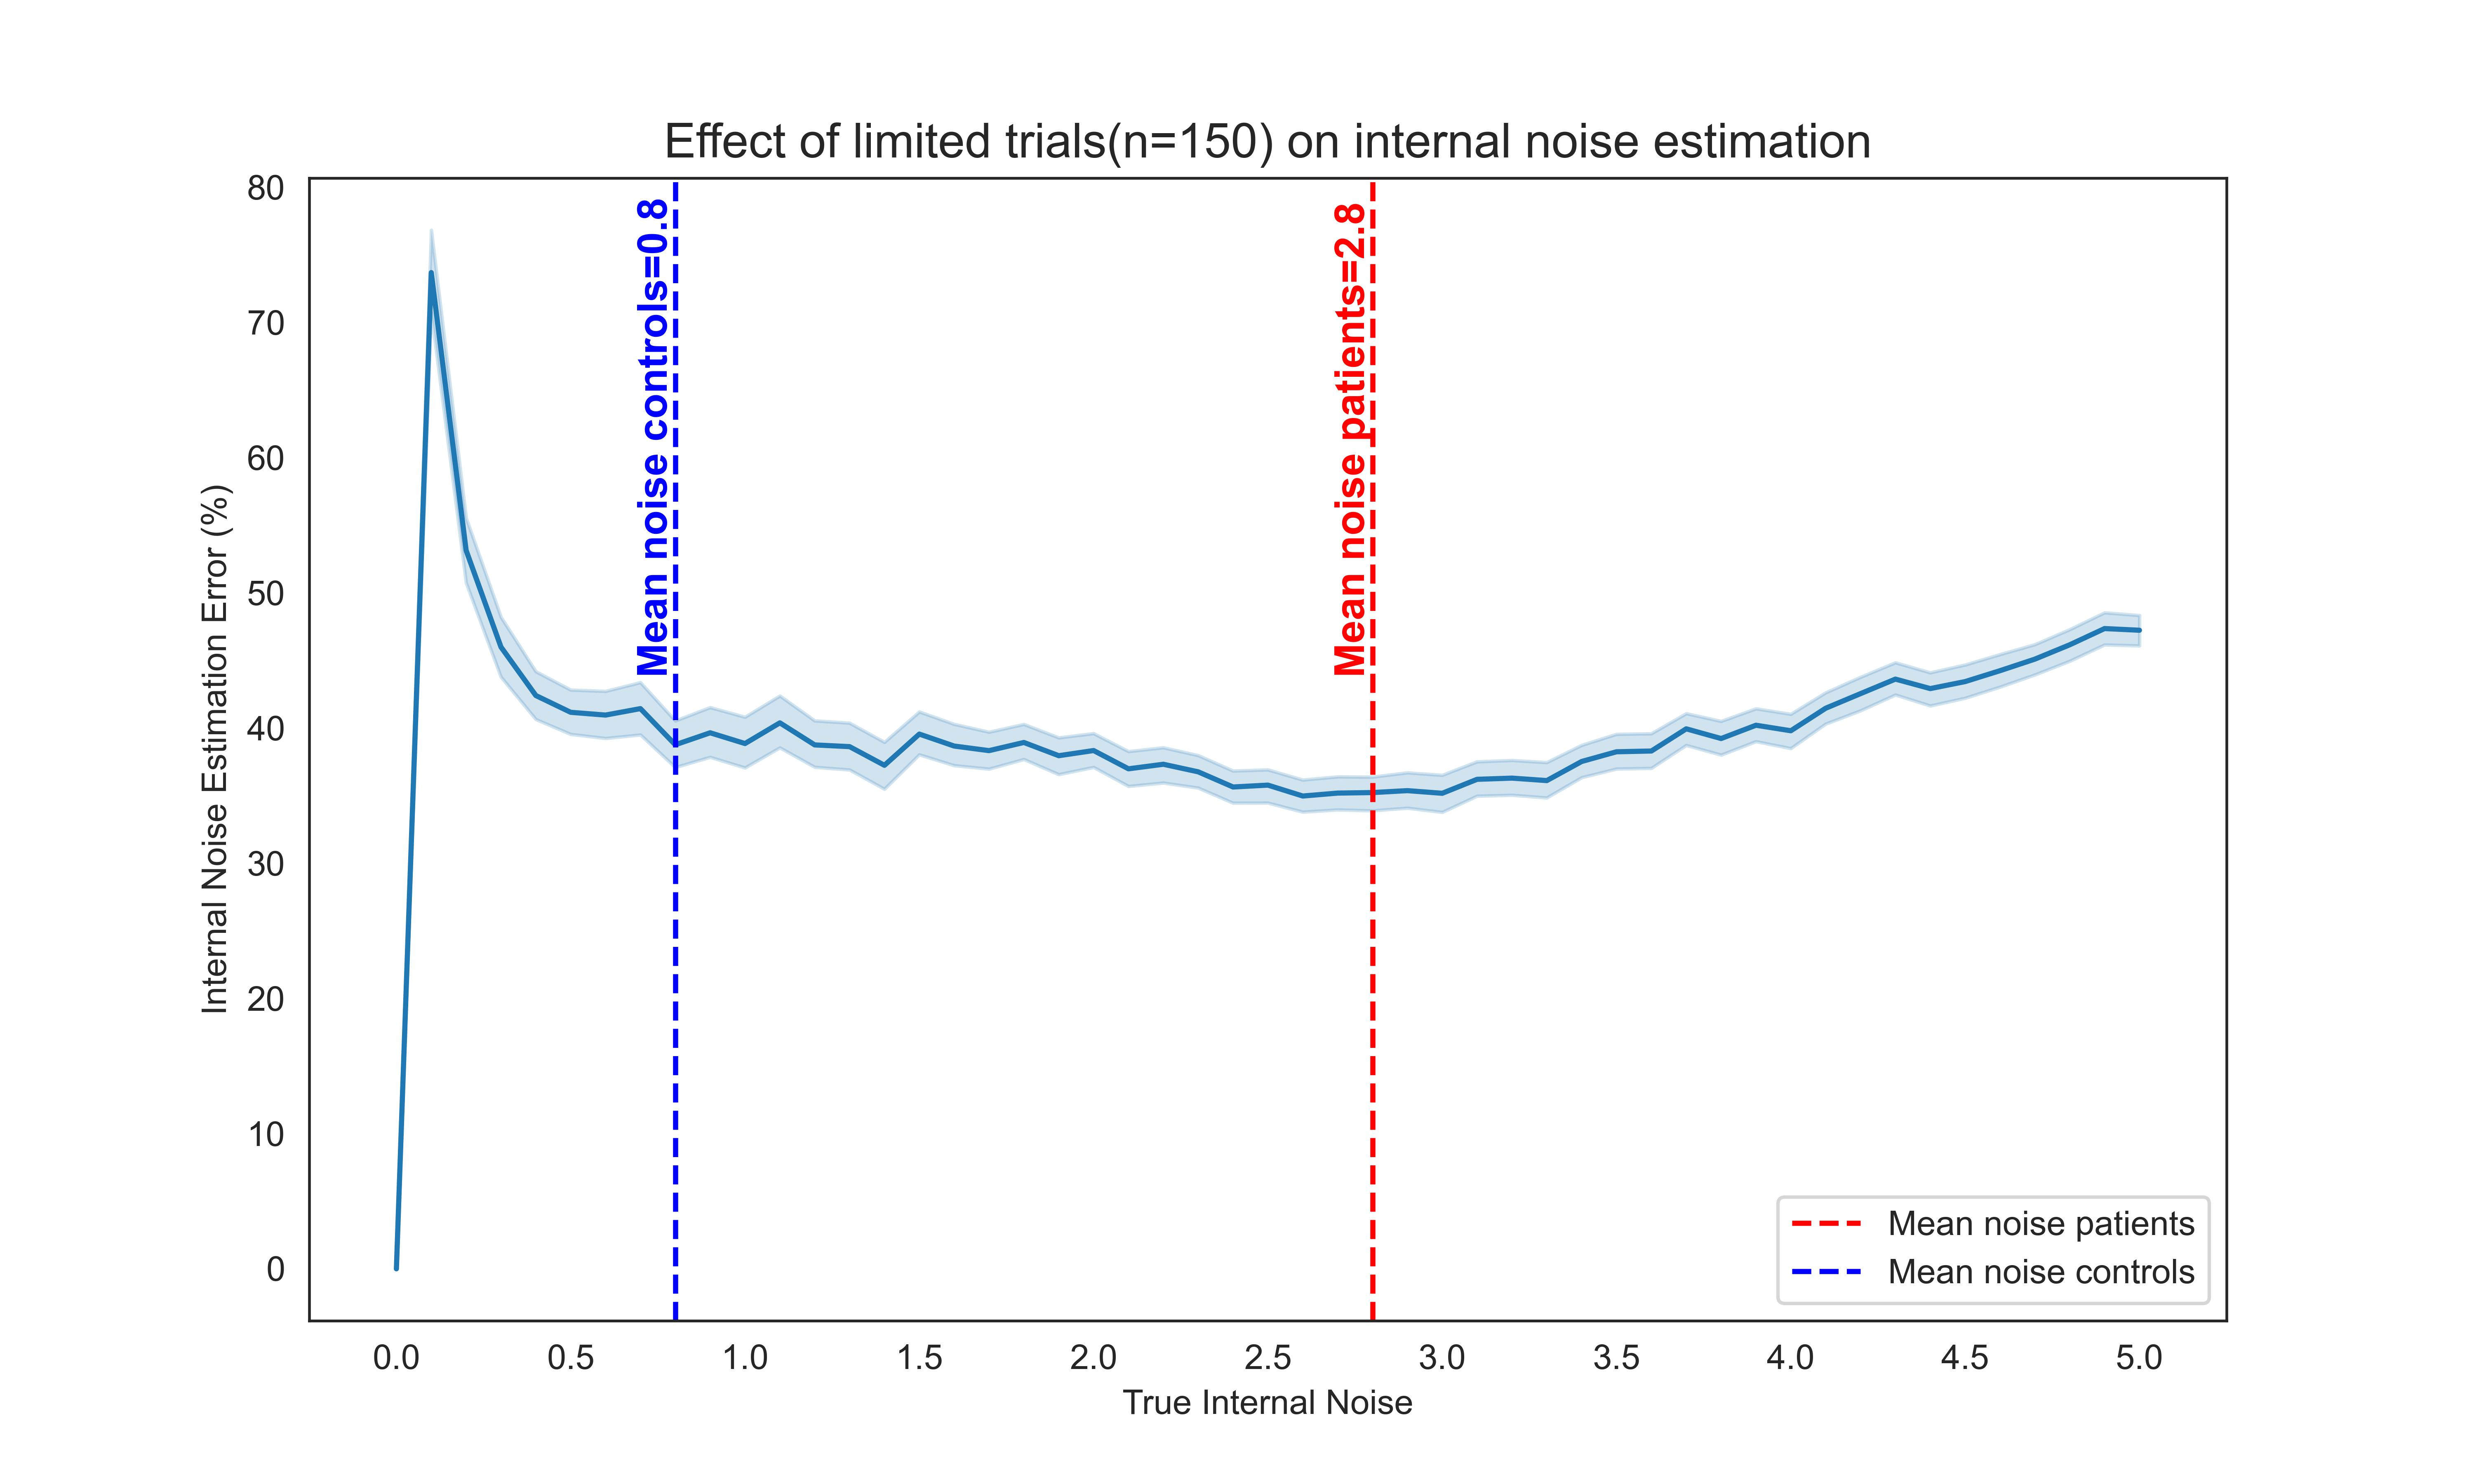
\includegraphics[width=15cm]{MainLayout/Images/chapter5/noise_150.jpg}
    \caption{Main Title for First Image \\ \small Subtitle for the first graphic.}
    \label{fig:noise_150}
\end{figure}

\begin{figure}[H]
    \centering
    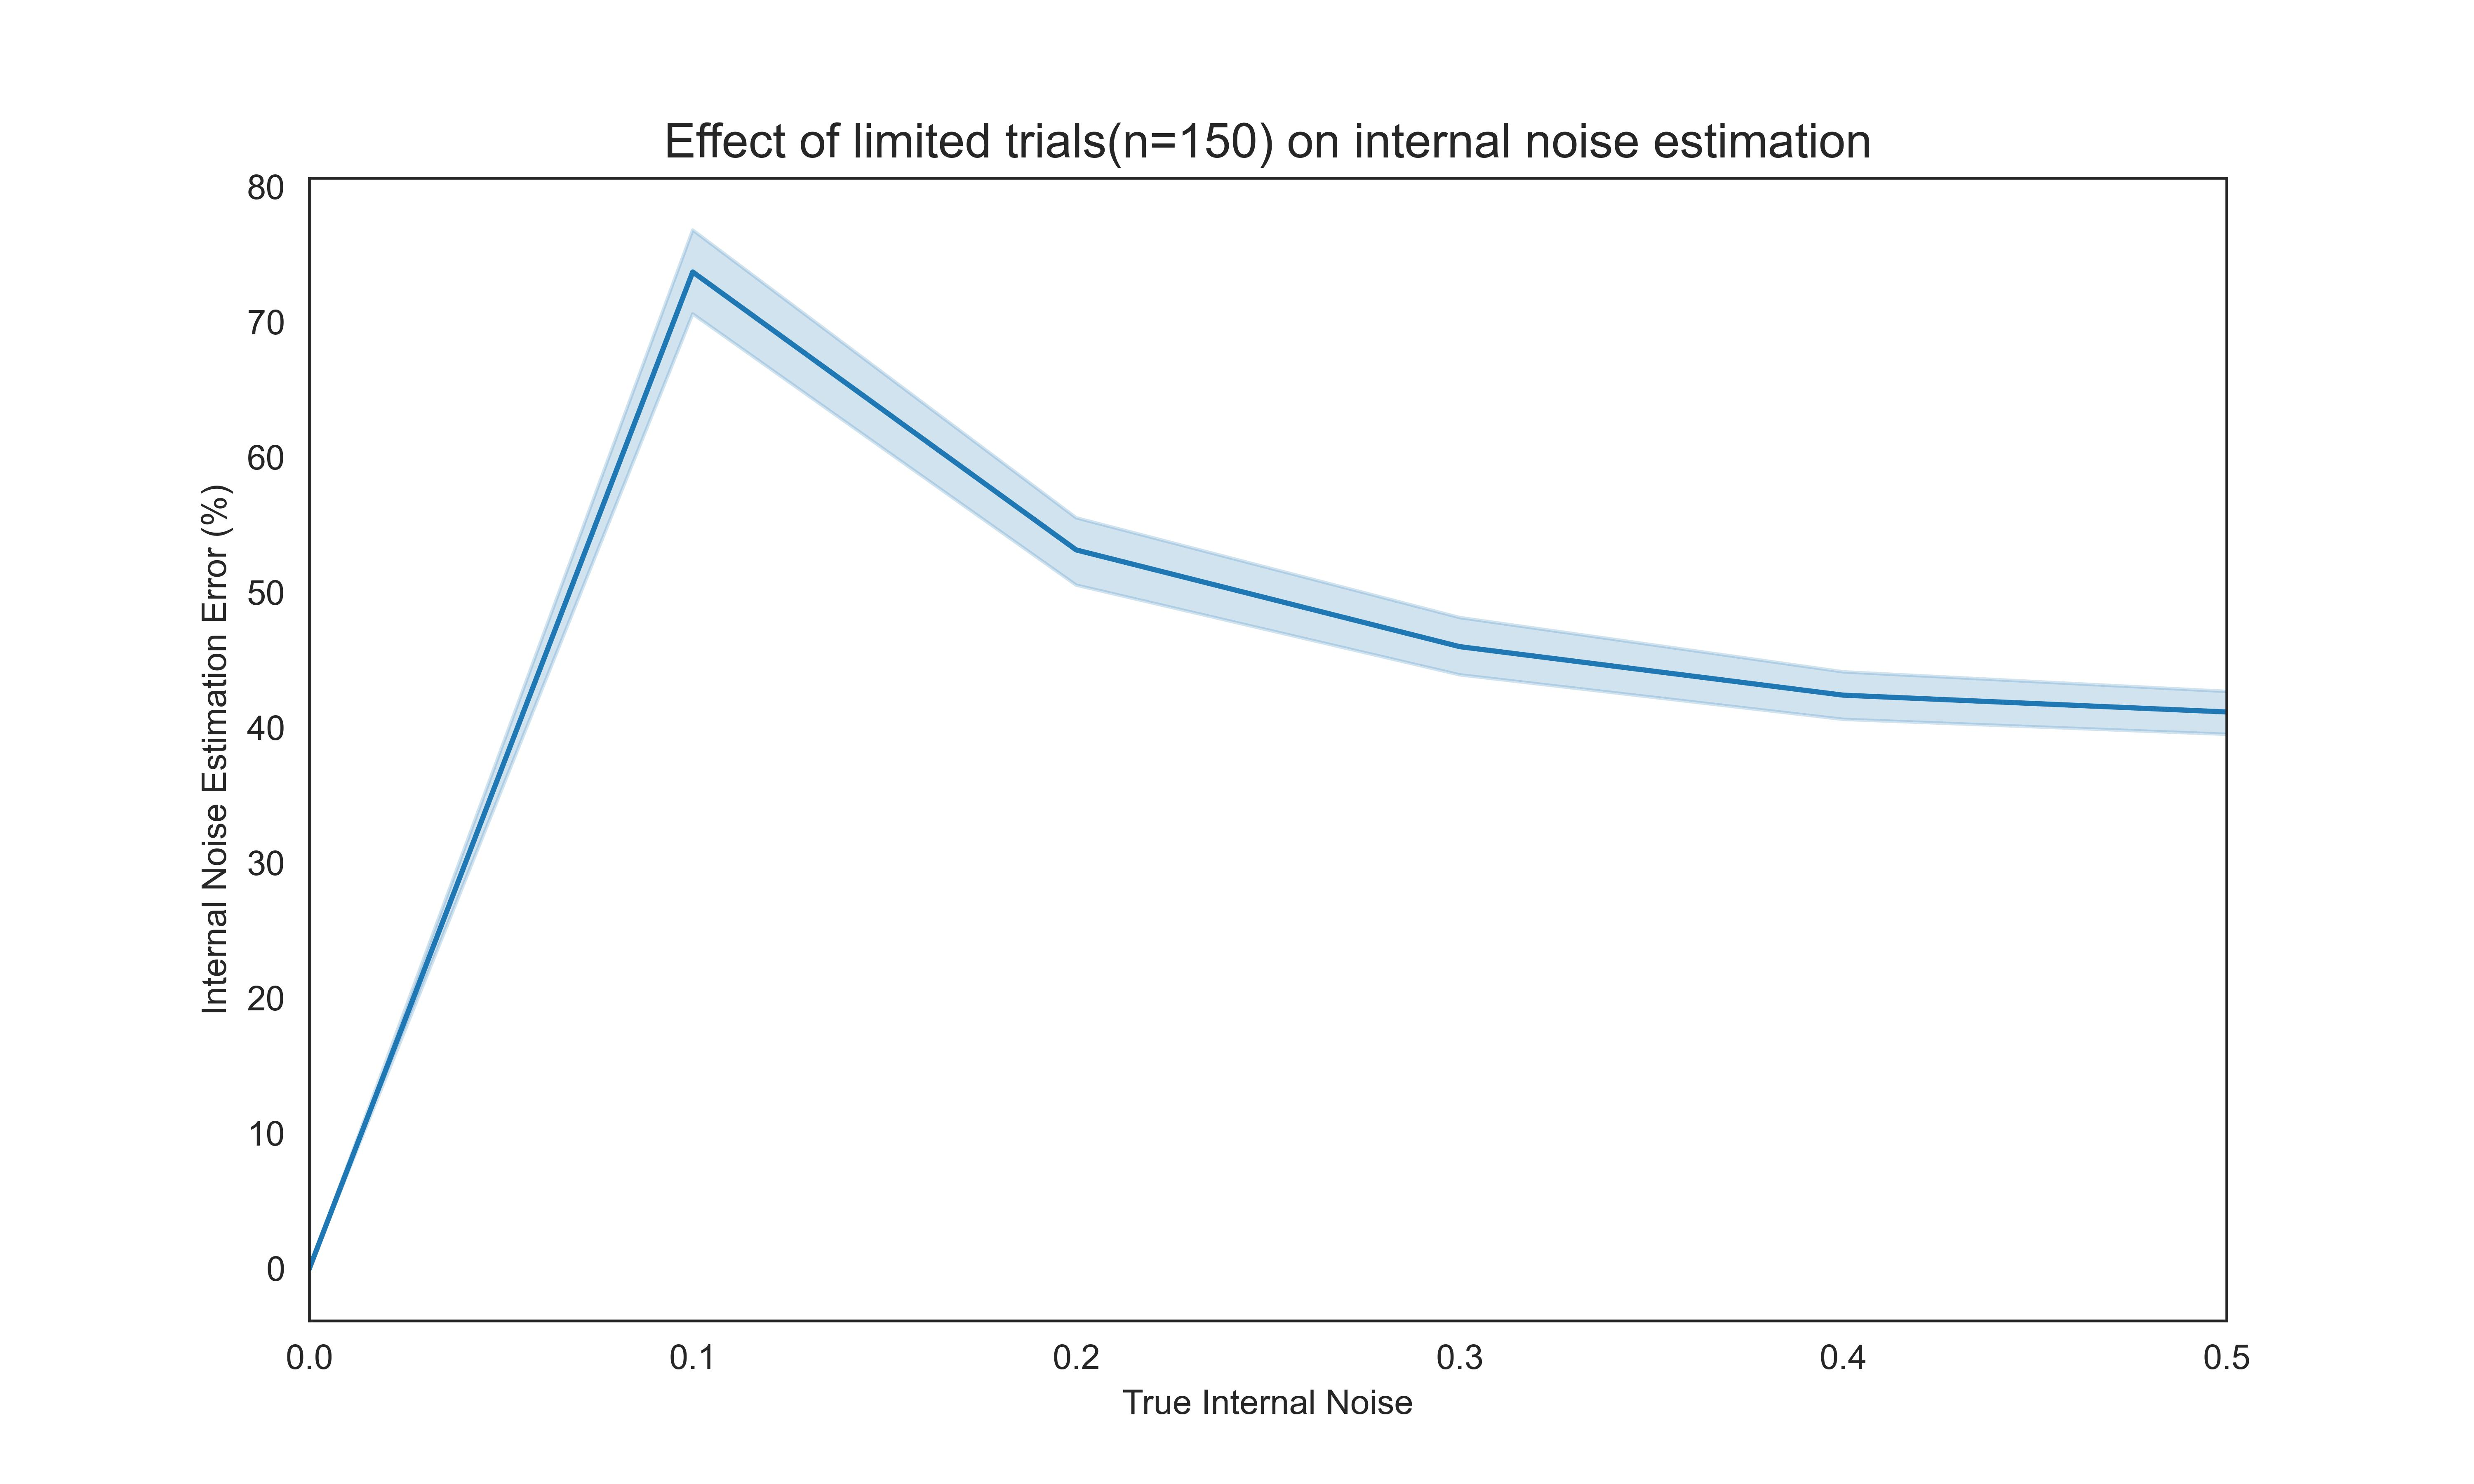
\includegraphics[width=15cm]{MainLayout/Images/chapter5/noise_150_0to05.jpg}
    \caption{Main Title for First Image \\ \small Subtitle for the first graphic.}
    \label{fig:noise_150_0to05}
\end{figure}


\section {Perseveration} 
As we already discussed in chapter \ref{chap2} is a cognitive phenomenon characterized by the repetitive execution of the same response, even when it is no longer appropriate or relevant to the task at hand, and is often linked to deficits in attentional control in decision making process and spatial neglect. From the perspective of the linear observer model and signal detection theory, participants exhibiting perseverative behavior no longer rely on their decision model to guide their responses. Instead of making choices based on their mental representation, they disengage from actively applying it to the stimuli. As a result, their responses become detached from stimulus evaluation, suggesting a lack of attentional control in determining which stimulus should be chosen.

\subsection {Perseveration a consequence of stroke} 
%It is possible that their excessive responses do not align with the average pathological profiles, leading to misclassification. 

By examining responses closely our patients responses, we observe that some stroke patients consistently chose the same stimulus across multiple trials without variation shown in figure \ref{fig:patient_responses}. which can be the result of attentional challenges following right-hemisphere stroke. This pattern has also been notably observed during speech and language therapy (SLT) sessions by therapists, further highlighting its clinical relevance. 

Several established tasks exist for quantifying perseveration, such as Object Alternation (OA) \cite{freedman_orbitofrontal_1998} and the Wisconsin Card Sorting Test (WCST) \cite{abbruzzese_performance_1996}, which are widely used in assessing cognitive rigidity in conditions like aphasia and schizophrenia. These tasks measure executive function impairments, including difficulty in adapting to rule changes and excessive response repetition. However, despite their use in broader neuropsychological research, they have not been systematically applied to evaluate prosody perception deficits after stroke. Investigating whether similar mechanisms of perseveration extend to prosodic processing could provide new insights into the relationship between executive function deficits and speech impairments in stroke patients.
\begin{figure}[H]
    \centering
    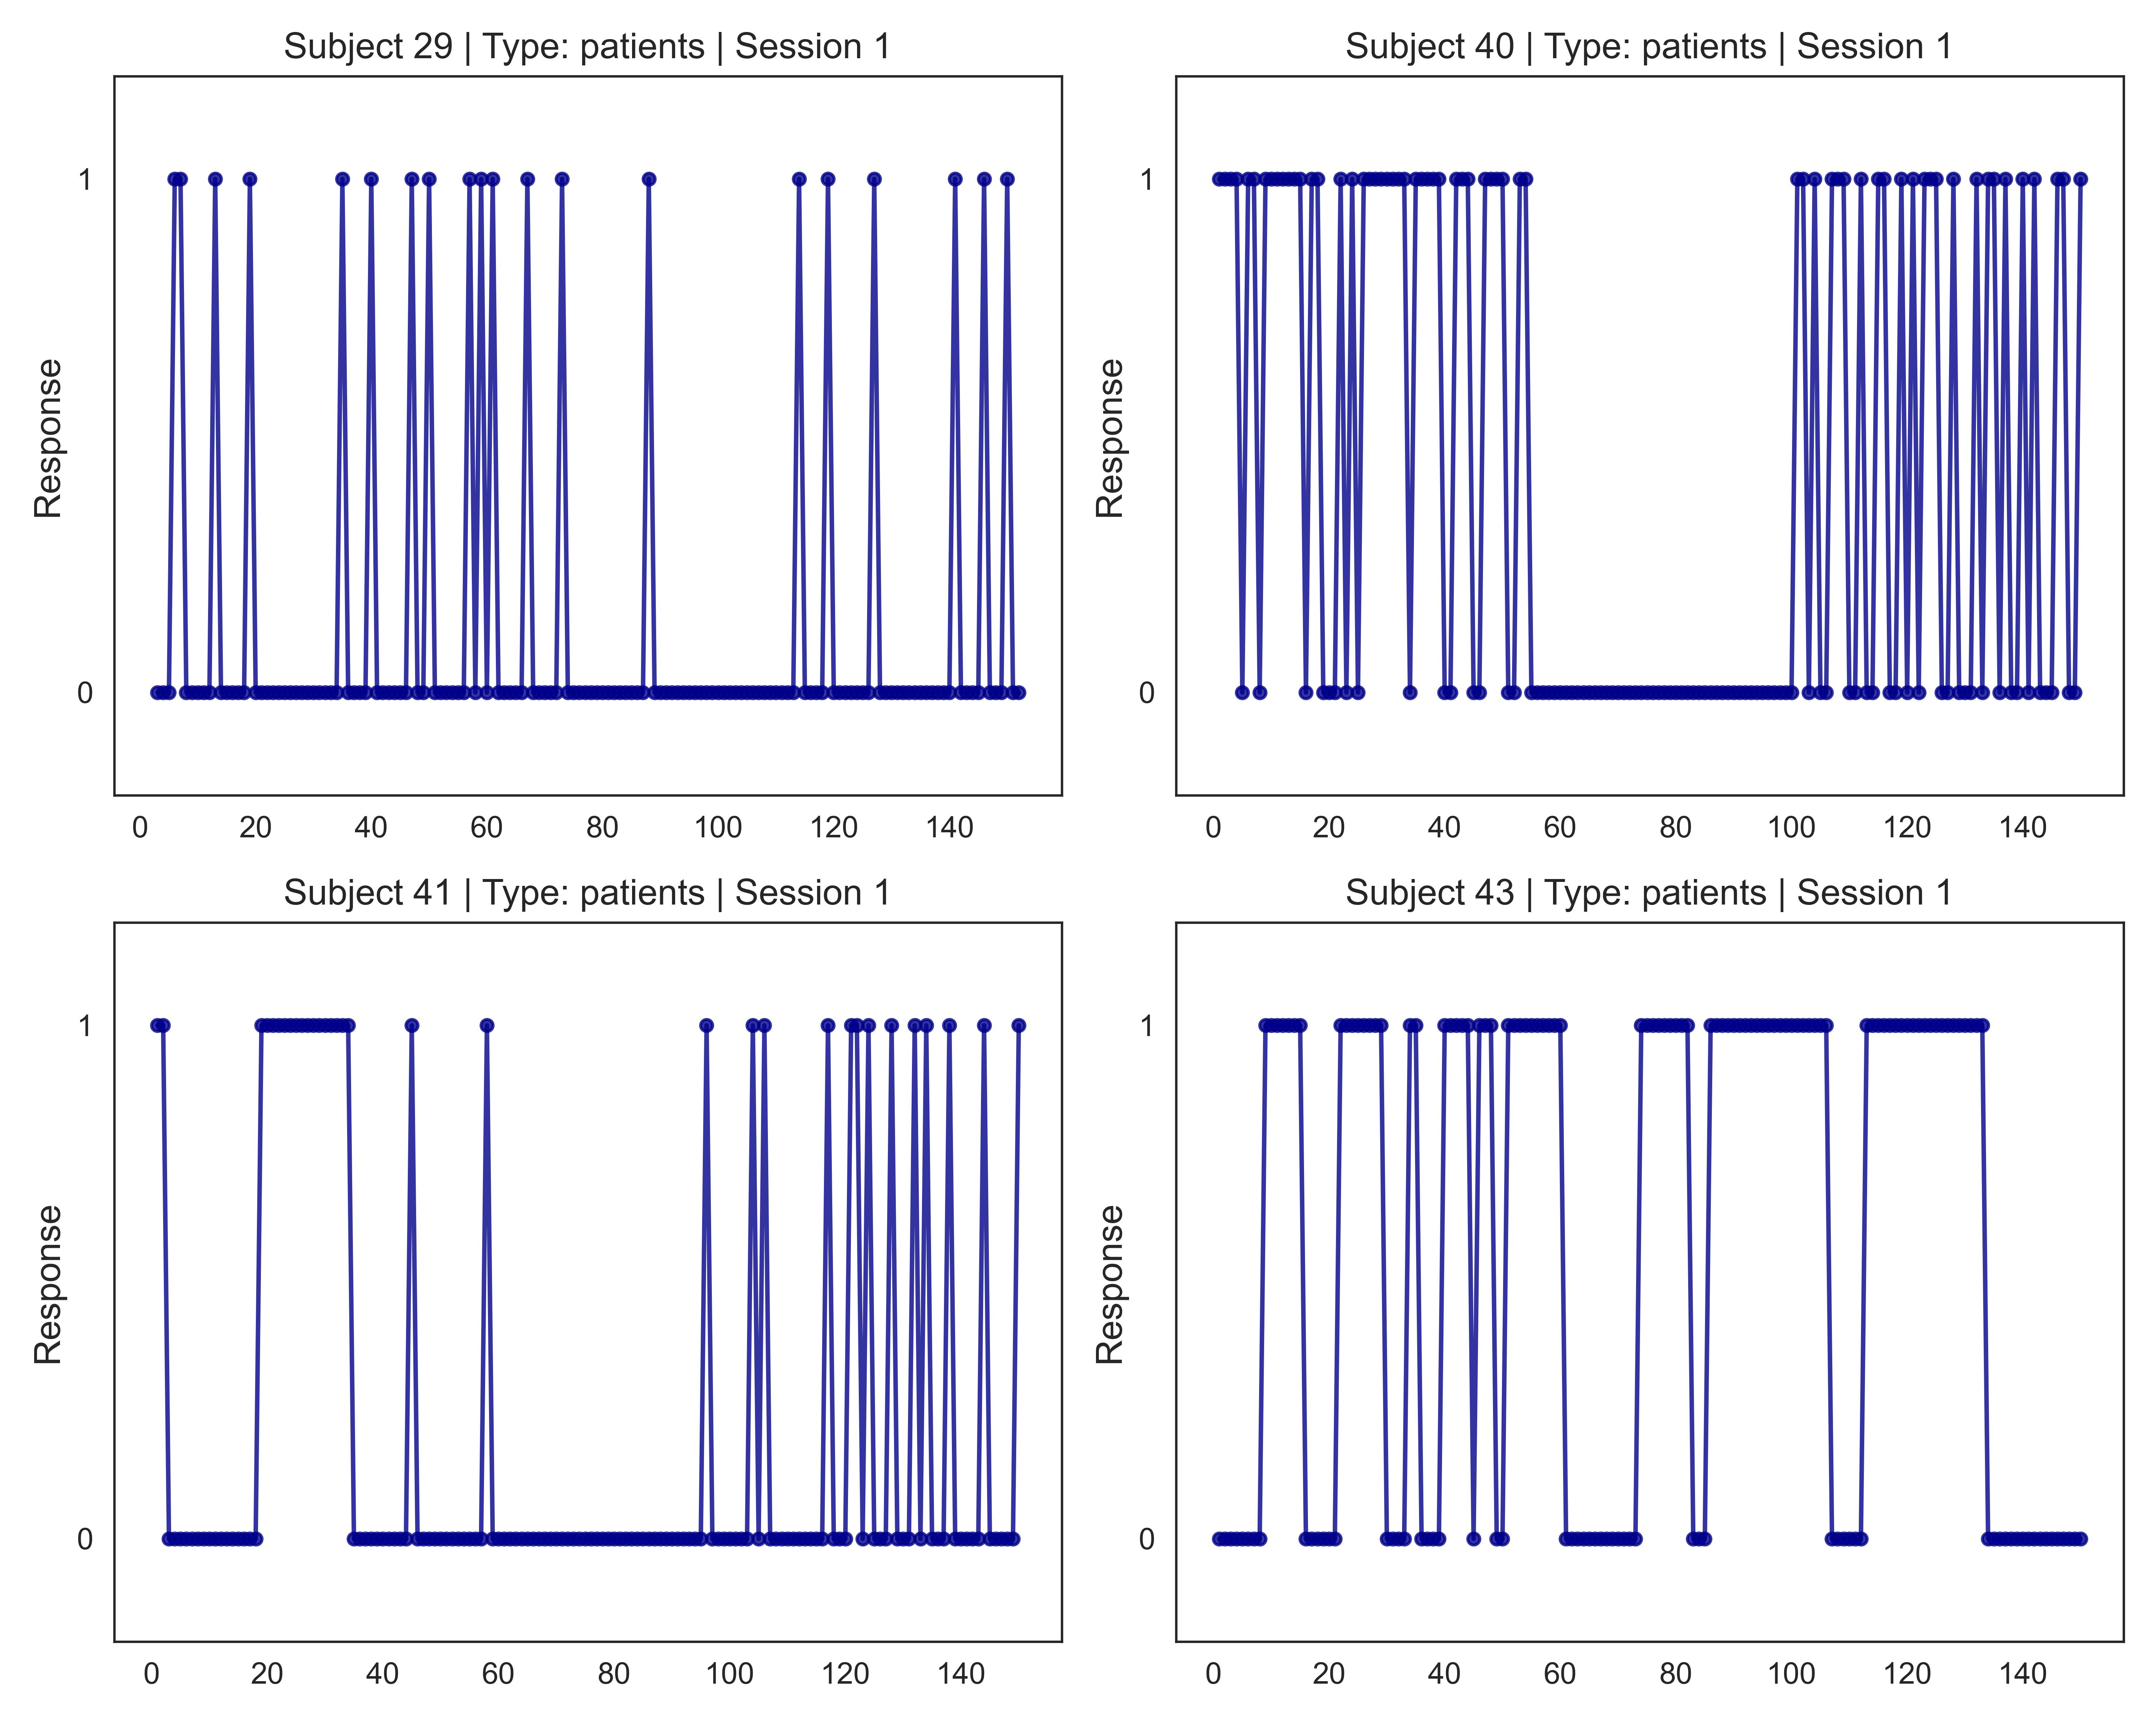
\includegraphics[width=15cm]{MainLayout/Images/chapter5/patient_responses.jpg}
    \caption{Main Title for First Image \\ \small Subtitle for the first graphic.}
    \label{fig:patient_responses}
\end{figure}

In the double-pass experiment, excessive responses may occur in repeated trials, potentially leading to false probabilities of agreement, making them appear to have high internal noise, despite their disengagement from the experiment. Conversely, if these behaviors do not manifest within the repeated trials, they may go undetected by internal noise estimates, leading to underestimation of internal noise. Additionally, because our kernel estimation relies on the average of responses, some patients may appear to have representations similar to controls, despite underlying perseverative tendencies. This raises the question of whether our regression-based method for classifcation images is truly optimal or if it leads to an over- or underestimation of their deficits.
In our experiment, we did not have the opportunity to directly measure participants' attention during the blocks. However, one way to estimate perseveration is by calculating the perseveration ratio, which involves identifying streaks of repeated responses within each participant, session, and block. Trials are marked as perseverative if they belong to a streak of 15 or more consecutive repeated responses. As shown in Figure \ref{fig:perseveration_block}, the perseveration ratio for patients (median = 0.64) is higher, particularly in the first and second blocks, compared to controls (median = 0.56). However, this analysis does not account for the interaction between the stimulus and the kernel, which may influence response patterns.

\begin{figure}[H]
    \centering
    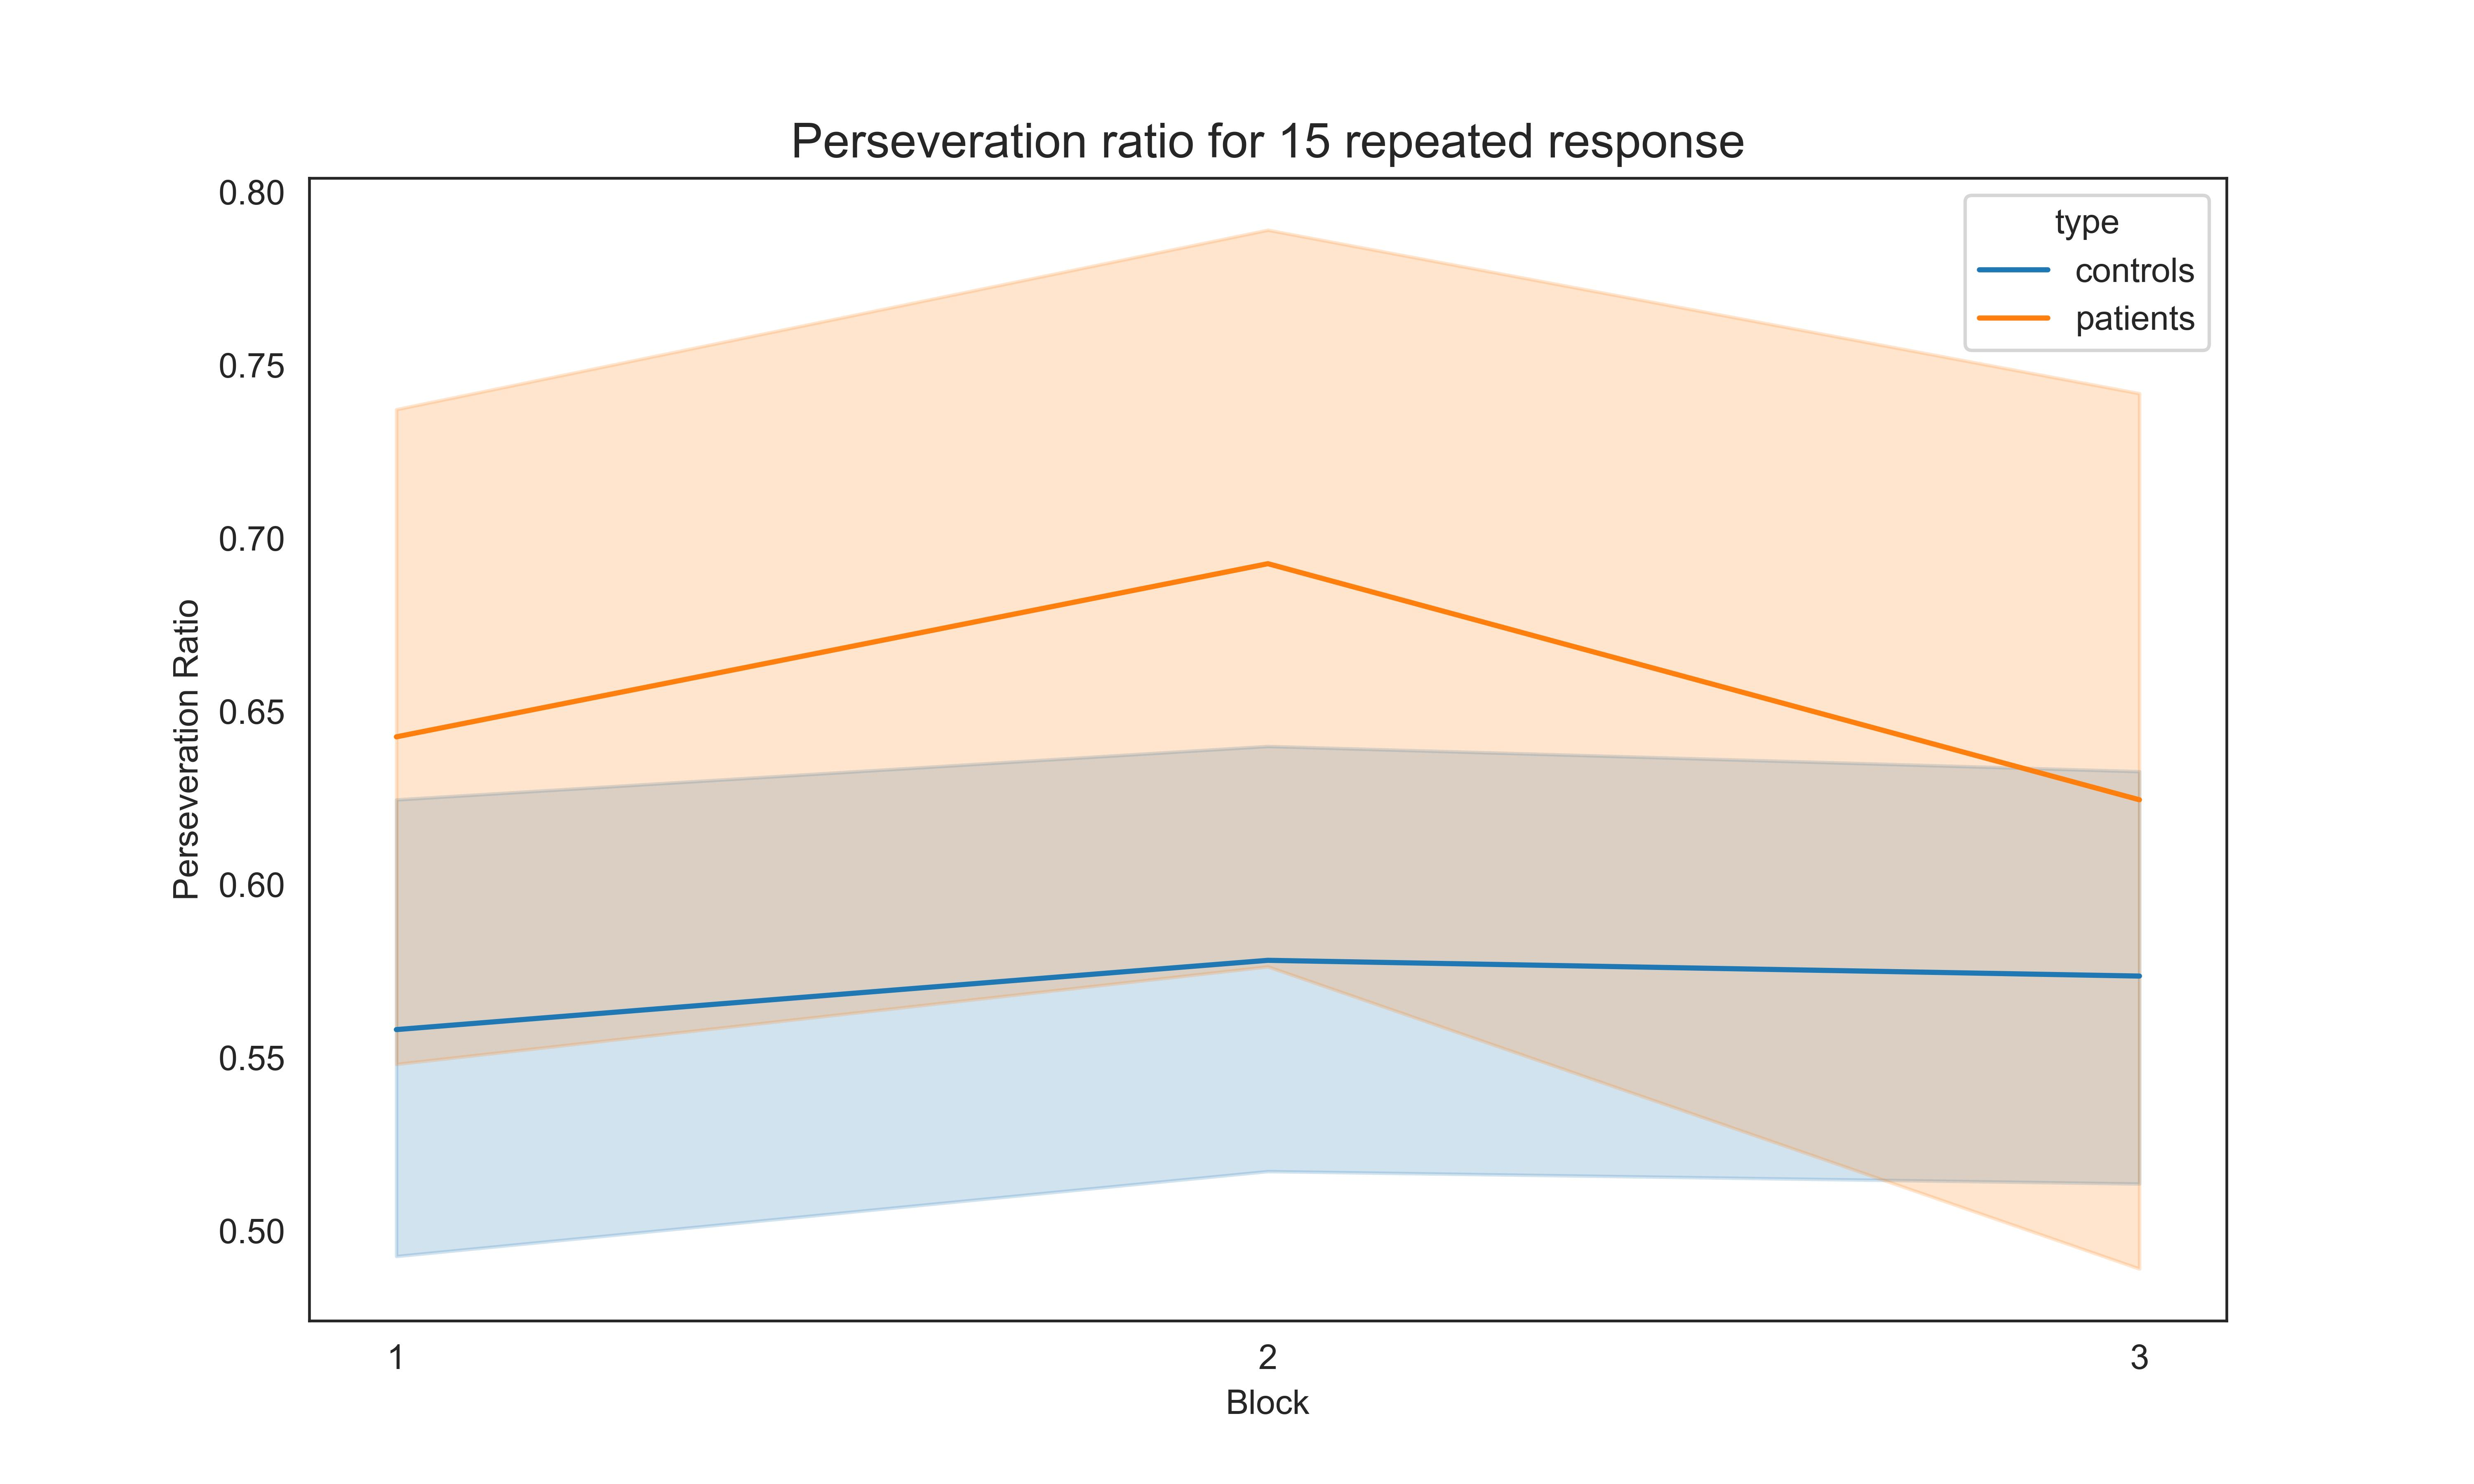
\includegraphics[width=15cm]{MainLayout/Images/chapter5/perseveration_block.jpg}
    \caption{Main Title for First Image \\ \small Subtitle for the first graphic.}
    \label{fig:perseveration_block}
\end{figure}


\subsection{Perseveration effects on kernel estimation}
Using the PALIN framework, we simulated a perseverating observer with a probability $p(a)$ of entering a perseverative phase and a probability $p(1-b)$ of remaining in that phase. These parameters were varied to increase the proportion of perseverative trials, simulating conditions where patients exhibit more repetitive behavior. In this simulation, the perseverating observer performs the same reverse correlation experiment as real participants, providing insights into how varying levels of perseveration (within a limited number of trials, n=150) influence the kernel correlation—the similarity between the true kernel of the observer and the estimated kernel. Like other simulations, this was repeated 1000 times to evaluate the estimation error.

As shown in Figure \ref{fig:kernel_perseverating_observer}, increasing the probability of remaining in the perseverative phase, $p(1-b)$ leads to a noticeable decline in kernel correlation, particularly for probabilities exceeding 0.5. Importantly, both patient and control groups in our study fall beyond this threshold, indicating that if participants remain in the perseverative phase for extended periods, the reliability of their kernel estimation significantly decreases due to increased error, suggesting that high levels of perseverative behavior can distort the relationship between true and estimated kernels.
\begin{figure}[H]
    \centering
    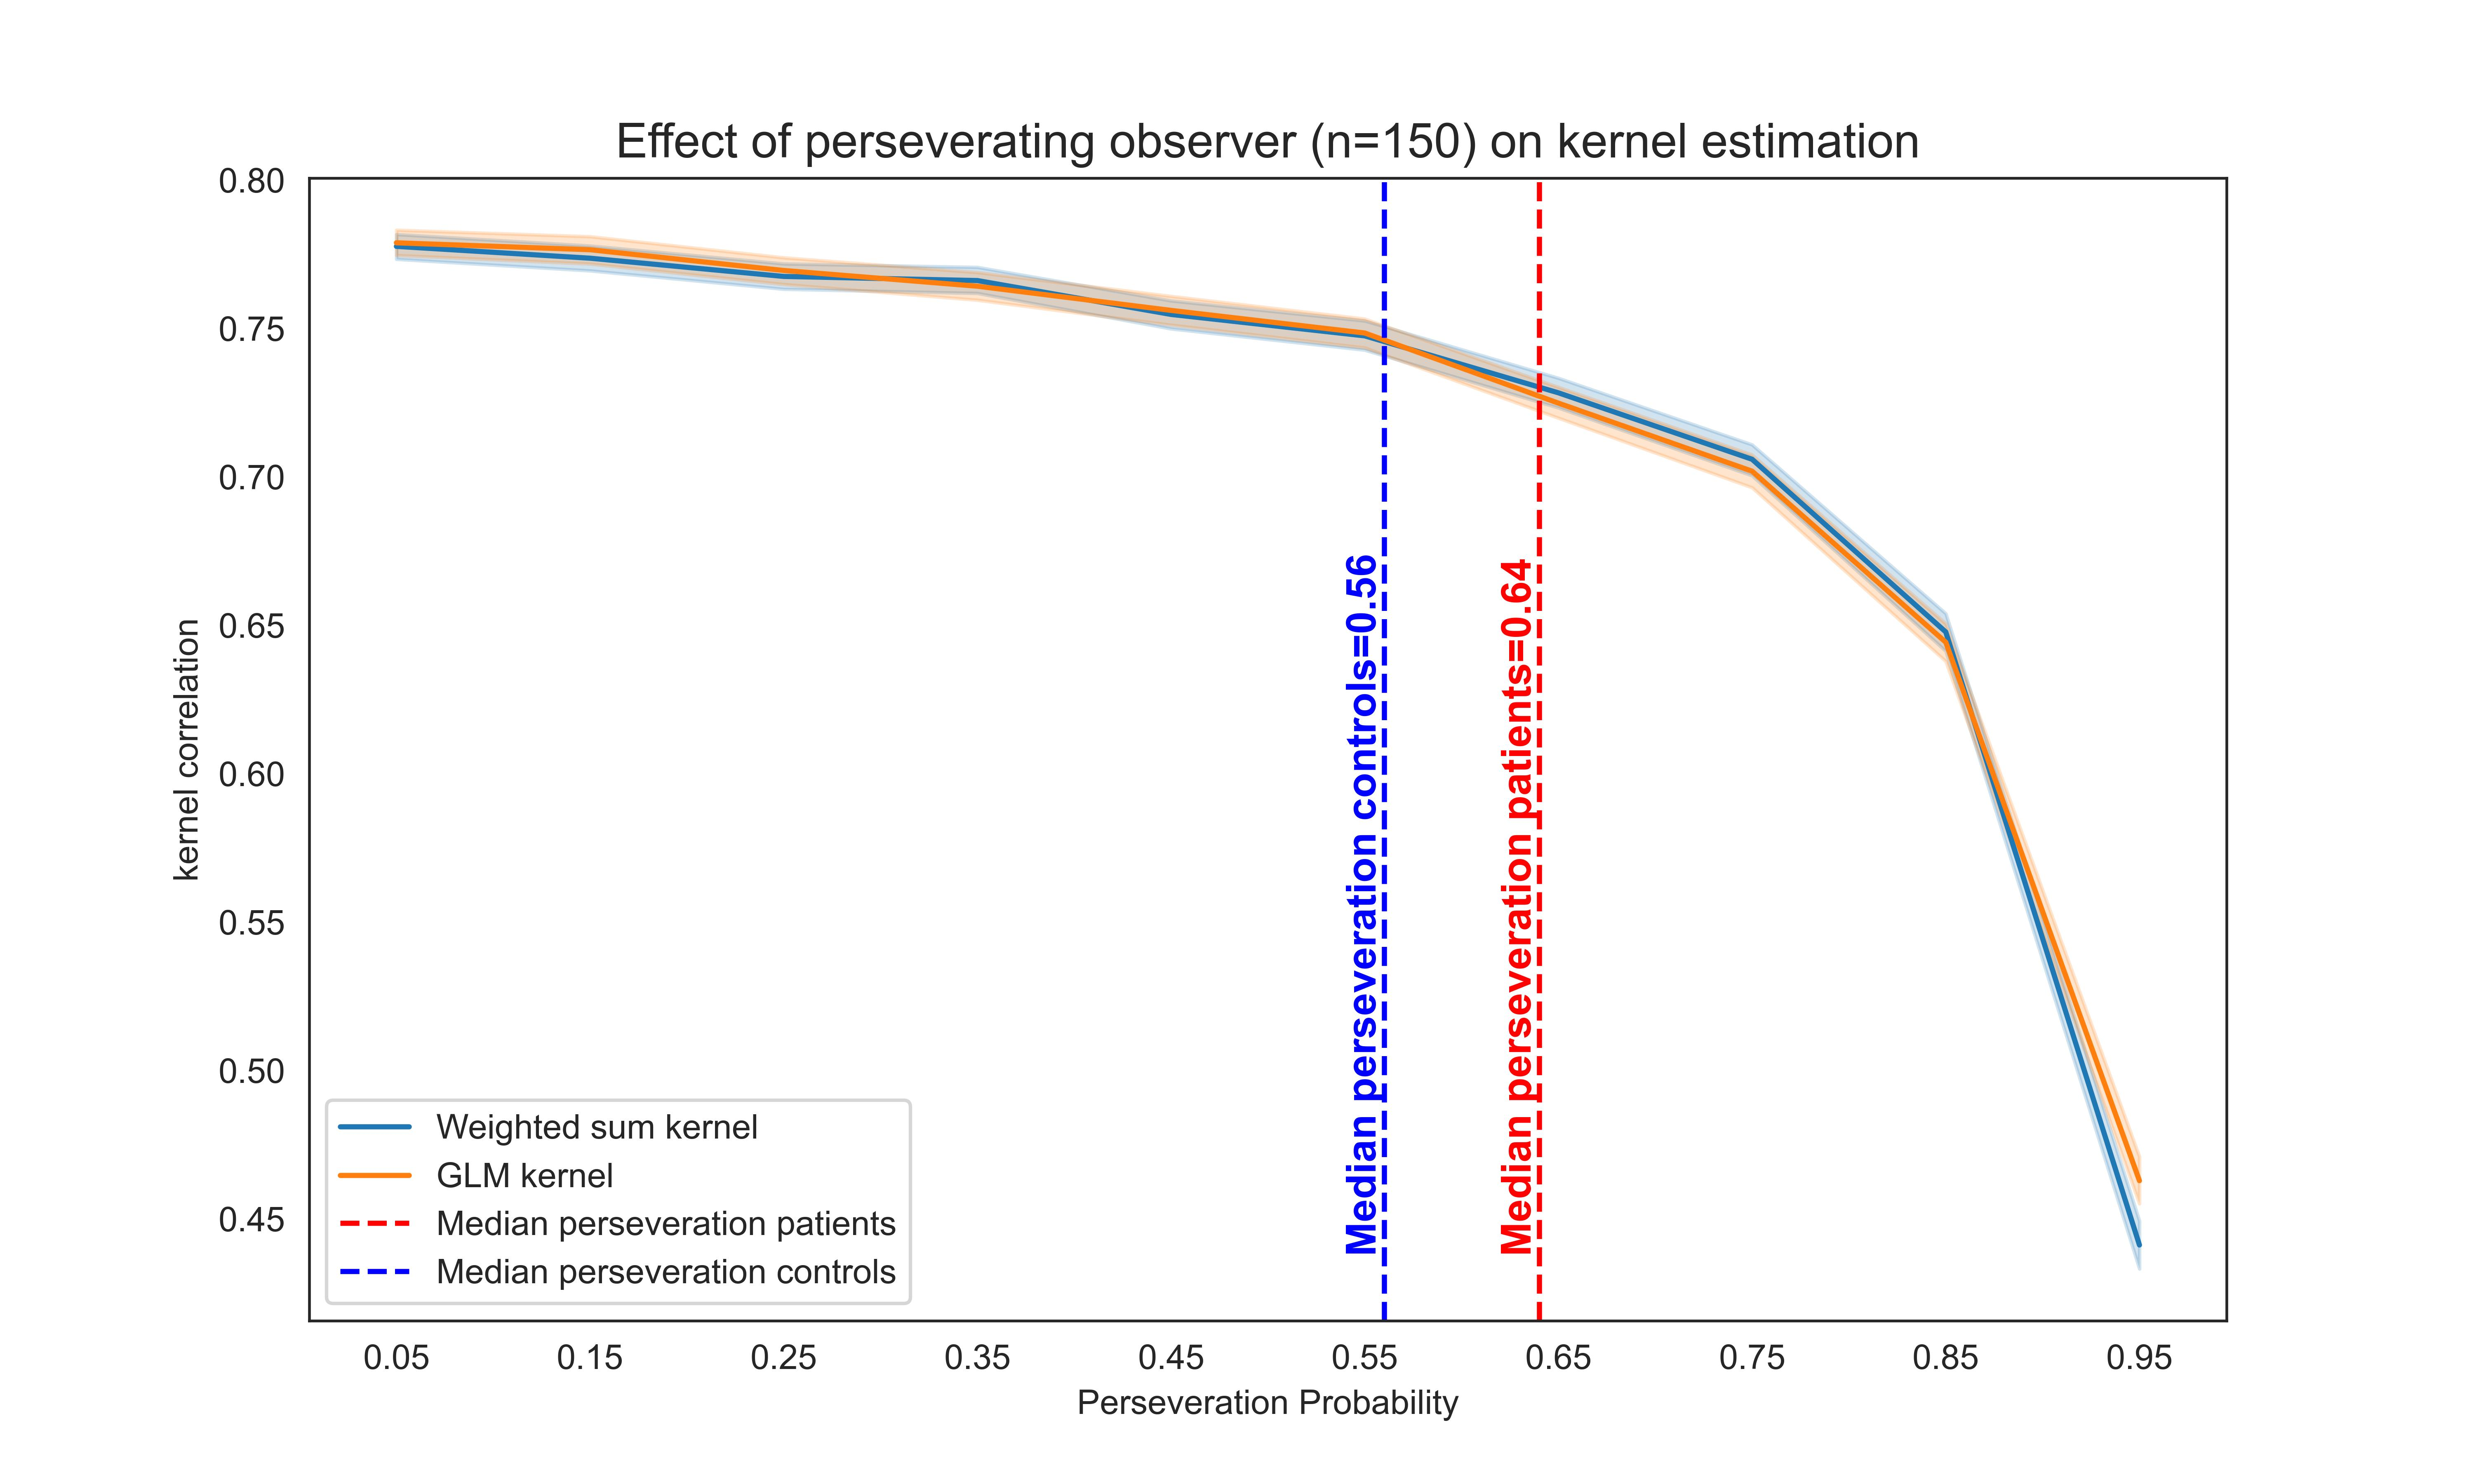
\includegraphics[width=15cm]{MainLayout/Images/chapter5/kernel_perseverating_observer.jpg}
    \caption{Main Title for First Image \\ \small Subtitle for the first graphic.}
    \label{fig:kernel_perseverating_observer}
\end{figure}

\begin{tcolorbox}[title=Palin Toolbox: Perseverating observer,
    colback=white!30!white, colframe=blue!80!white]

\begin{minted}[fontsize=\tiny]{python}
# Observer parameters define kernel type, internal noise range, decision criteria, 
# and state transition probabilities (for perseveration).
observer_params = {'kernel': ['random'],  'internal_noise_std': np.arange(1,5,0.5), 'criteria': [0], 
    'transition_matrix': [[[0.9, 0.1], [beta, 1 - beta]] for beta in beta_values]}
# Experiment parameters include trial counts, double-pass trials, stimulus features, 
# and external noise level.
experiment_params = {'n_trials':[150], 'n_repeated':[50], 'trial_type': [Int2Trial],
                     'n_features': [7],'external_noise_std': [100]}
# Analyzer parameters for internal noise use the Double Pass method.
analyser_params_noise = {'internal_noise_extractor':[DoublePass],
                   'agreement_model_file':['agreement_model_large.csv']}   
# Analyzer parameters for kernel estimation use ClassificationImage and GLMKernel methods.
analyser_params_kernel = {'kernel_extractor': [ClassificationImage,GLMKernel],'distance': ['CORR']}
# Simulate internal noise estimation for perseverating observers.
sim_in_per = Sim(DoublePassExperiment, experiment_params,  PerseveratingObserver, observer_params, 
                 InternalNoiseValue, analyser_params_noise)
# Simulate kernel estimation for perseverating observers.
sim_kernel_per = Sim(DoublePassExperiment, experiment_params,  PerseveratingObserver, observer_params, 
                 KernelDistance, analyser_params_kernel)
sim_kernel_perseveration_df = sim_kernel_per.run_all(n_runs=1000) 
sim_in_perseveration_df = sim_in_per.run_all(n_runs=1000)
\end{minted}

\end{tcolorbox}
\subsection{Perseveration effects on internal noise estimation}
The percentage error in internal noise estimation can also be evaluated for a perseverating observer to determine whether increasing the probability of perseveration impacts estimation accuracy. As shown in Figure \ref{fig:noise_perseverating_observer}, an observer with no perseveration exhibits an estimation error of approximately 40\%, consistent with previous findings in Figures \ref{fig:noise_150} and \ref{fig:internal_noise}. However, as the probability of perseveration increases, the estimation error initially rises gradually before accelerating sharply beyond a threshold of 0.55. Notably, our patient group falls beyond this limit, indicating that higher perseveration levels contribute to significantly greater internal noise estimation errors. This suggests that perseveration disrupts the reliability of internal noise estimation, making it more challenging to accurately capture perceptual variability in perseverating individuals.

\begin{figure}[H]
    \centering
    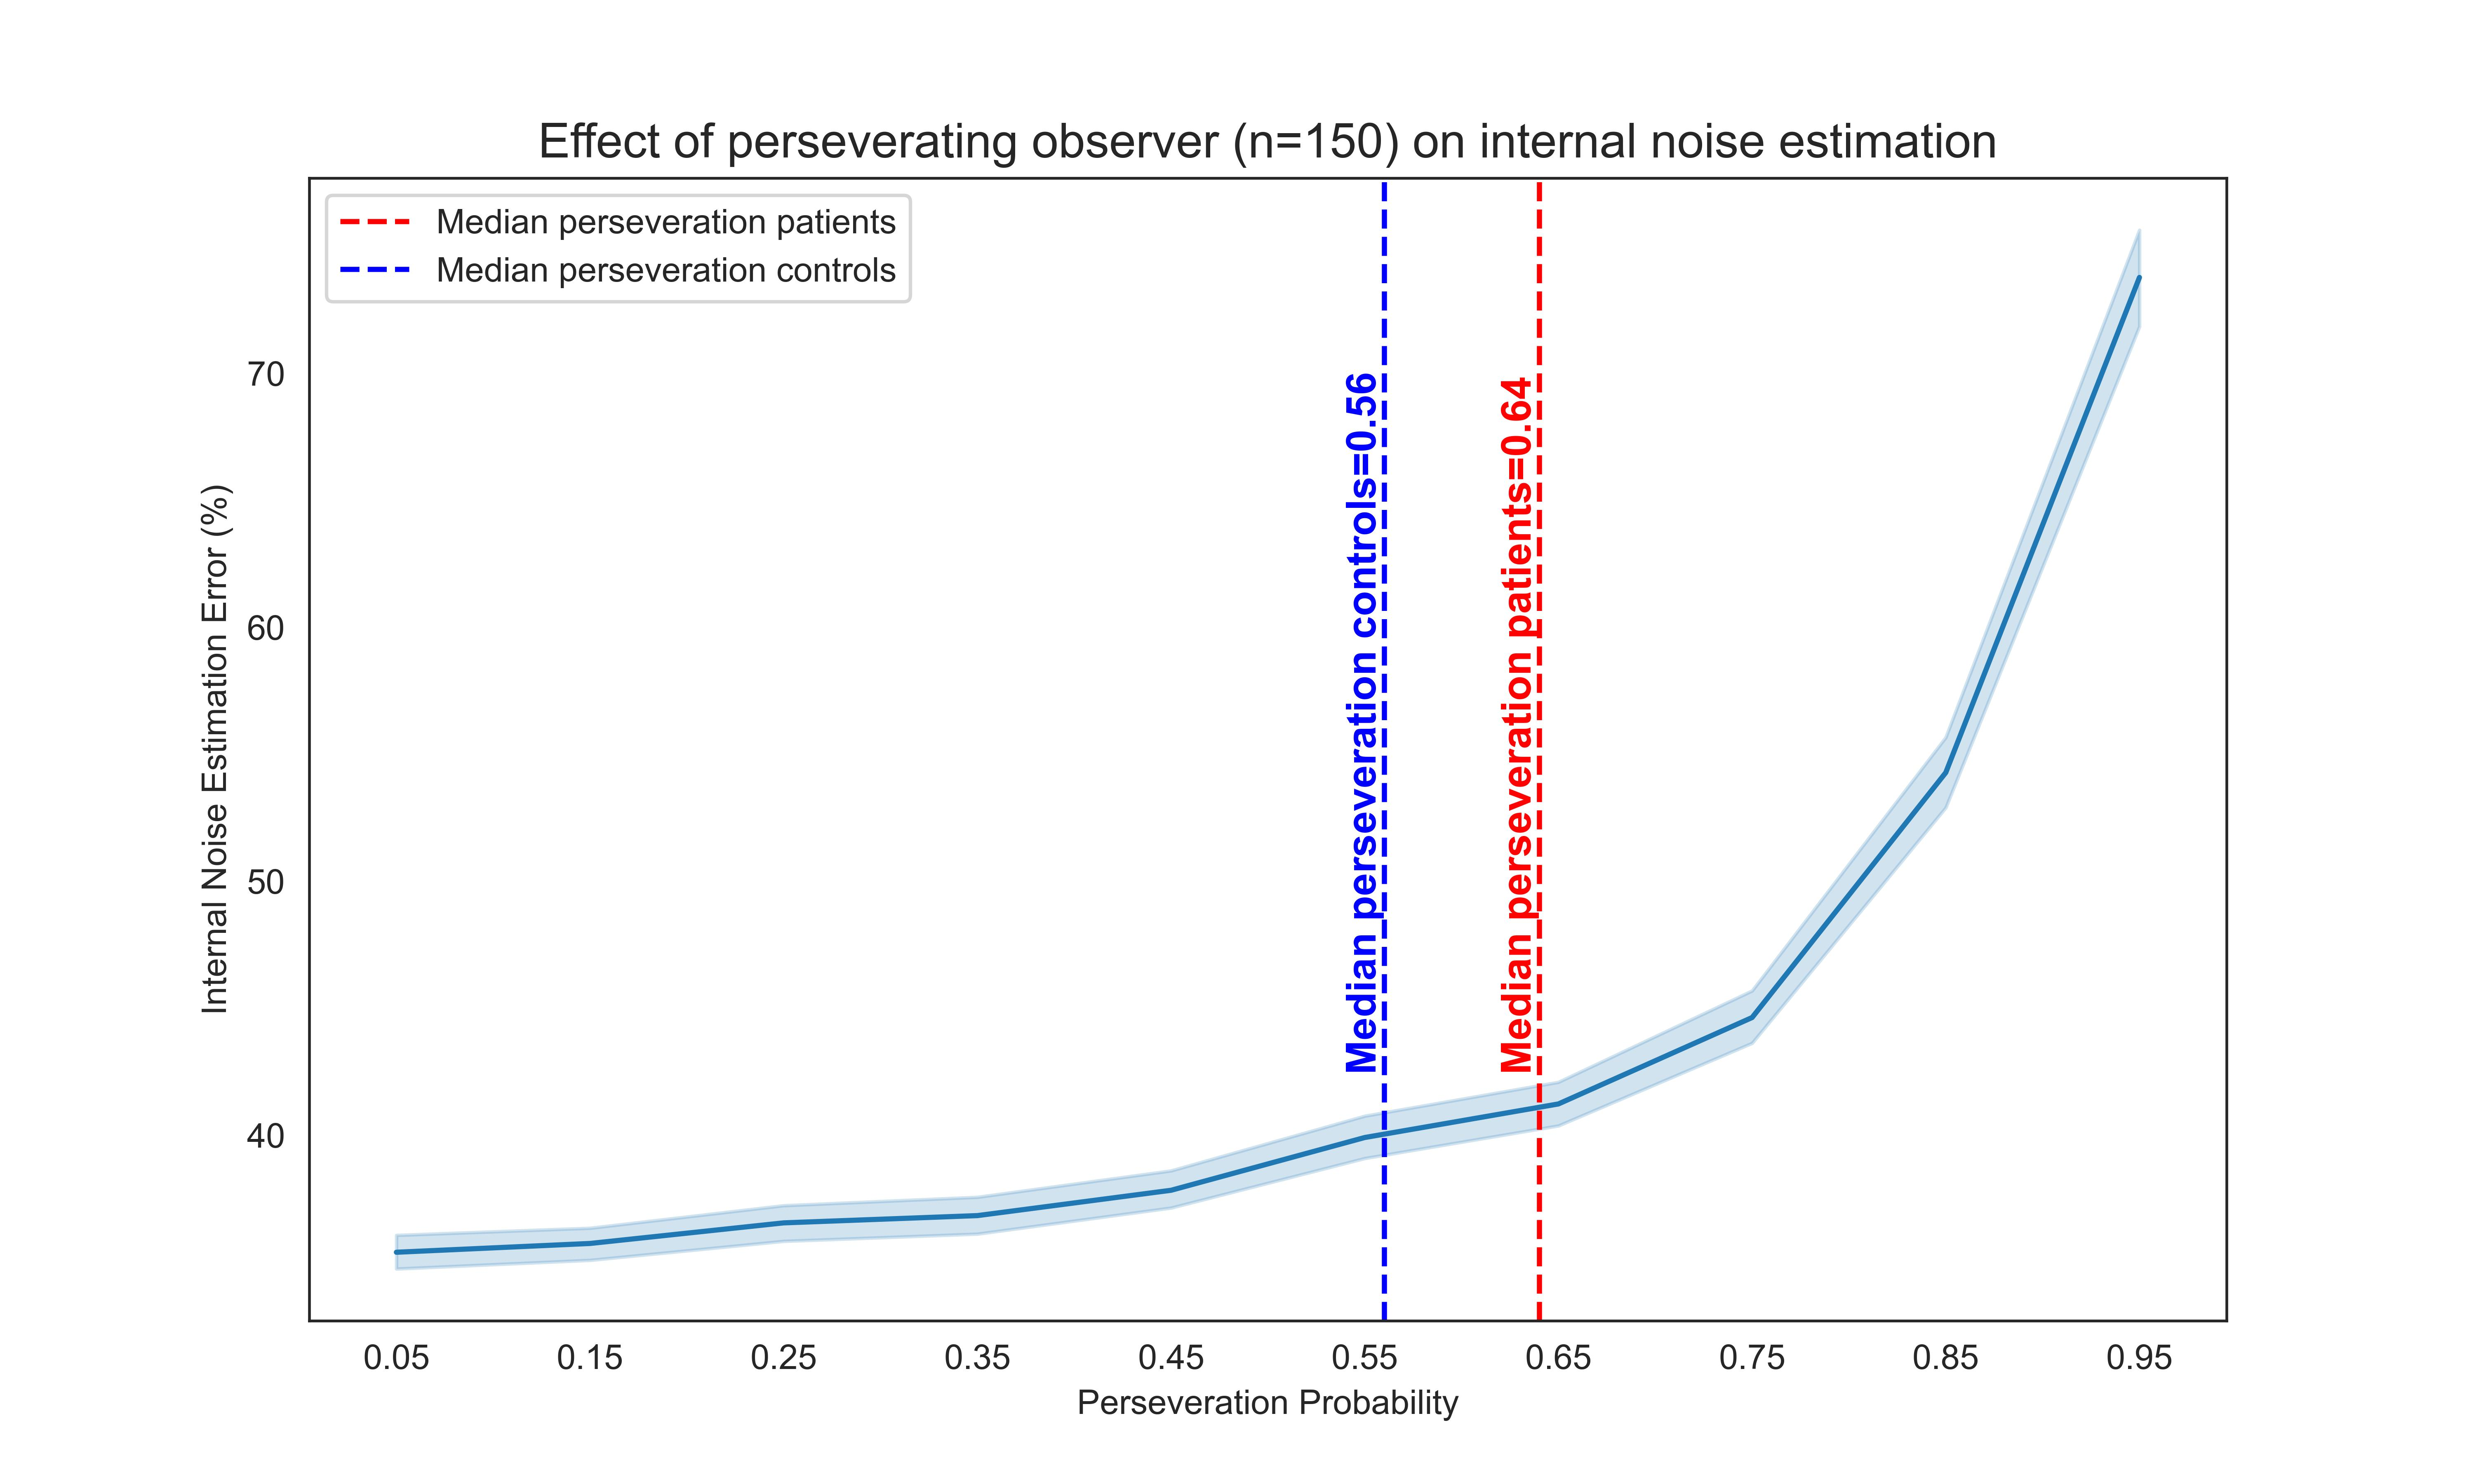
\includegraphics[width=15cm]{MainLayout/Images/chapter5/noise_perseverating_observer.jpg}
    \caption{Main Title for First Image \\ \small Subtitle for the first graphic.}
    \label{fig:noise_perseverating_observer}
\end{figure}

As shown in Figure \ref{fig:overestimation_noise}, even at low levels of internal noise, a perseverating observer consistently exhibits either overestimation or underestimation of noise. This occurs because perseveration reduces response variability, leading to biased noise estimates that depend on the level of perseveration. Higher probabilities of perseveration ($\beta$) amplify this bias, causing greater deviations between true and estimated noise. At low true noise levels (<1), the bias is particularly pronounced due to naturally low variability, which perseveration further reduces. Additionally, higher ($\beta$) increases variability in estimates, as shown by the widening shaded regions in the simulations.

\begin{figure}[H]
    \centering
    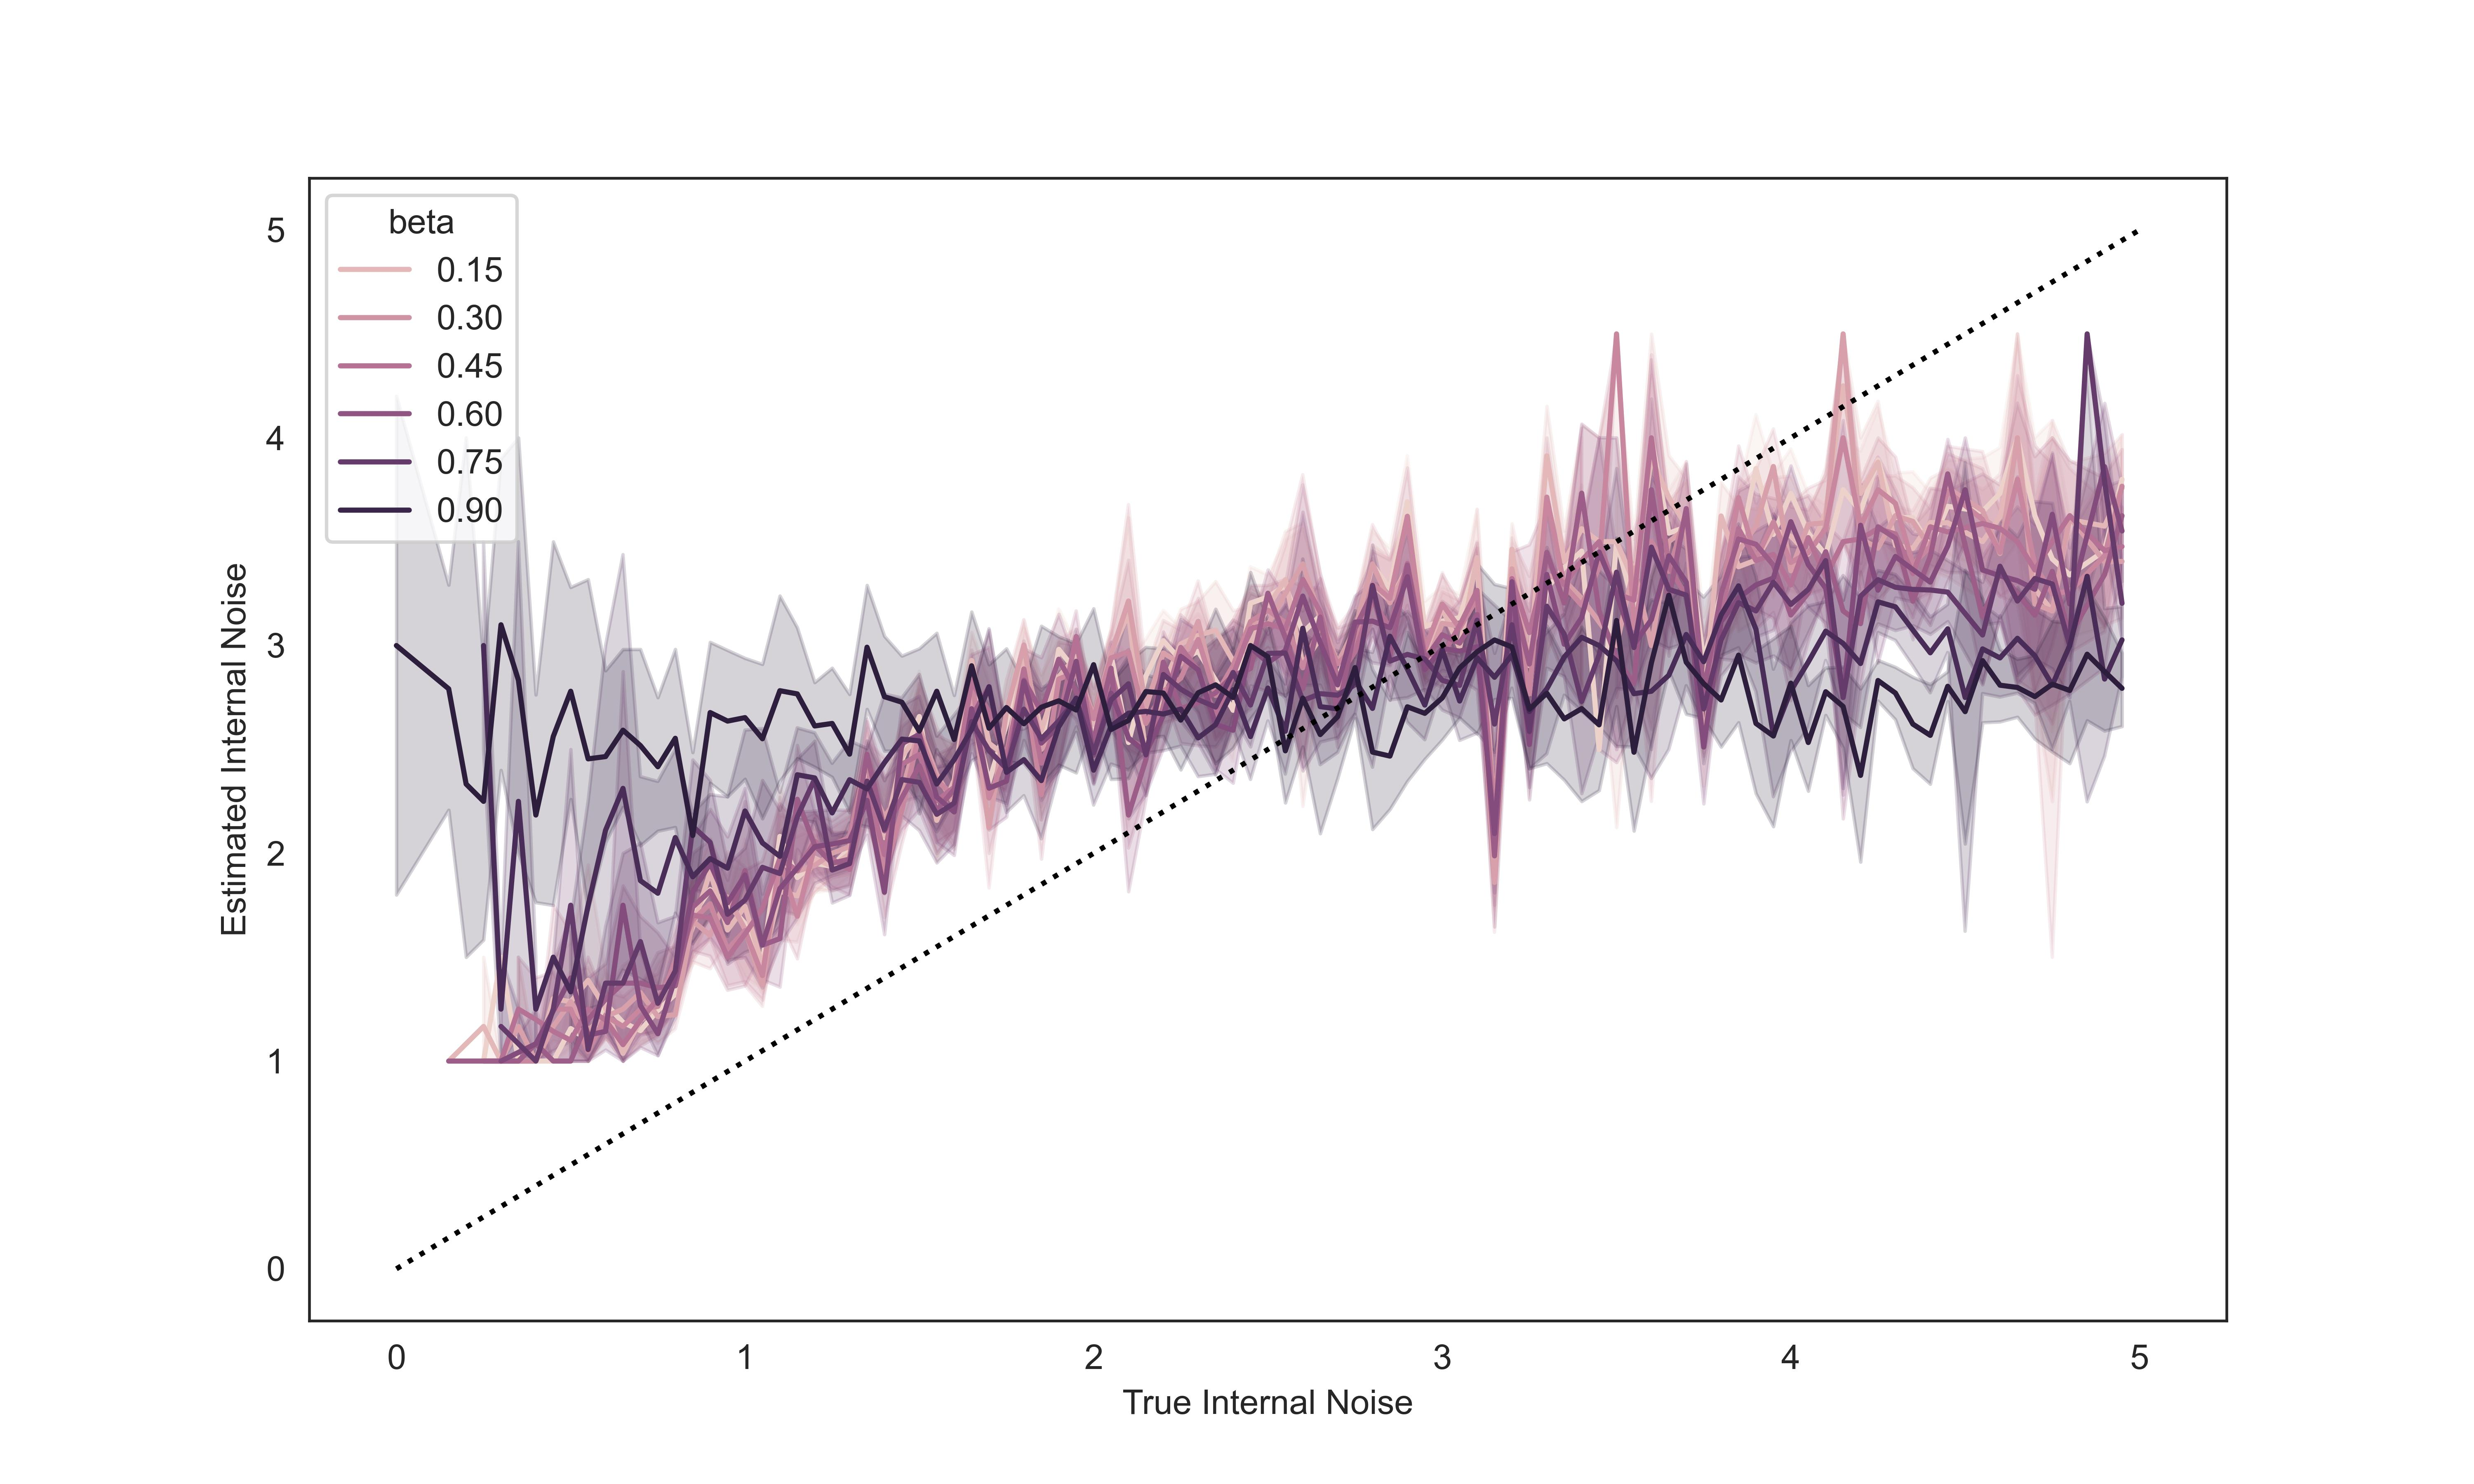
\includegraphics[width=15cm]{MainLayout/Images/chapter5/overestimation_noise.jpg}
    \caption{Main Title for First Image \\ \small Subtitle for the first graphic.}
    \label{fig:overestimation_noise}
\end{figure}


\section {Problem statement} 
In this chapter, we have identified two key challenges that affect the reliability of our methods for estimating internal noise and mental representations: the limited number of trials and perseveration. The limited trial count imposes constraints on the precision of estimations, particularly at higher noise levels, while perseveration disrupts response variability, leading to biased and inconsistent results. These two issues highlight critical limitations in our current approach, which compromise the accuracy and interpretability of the estimations.

In the next chapters, we aim to explore alternative methods that are less sensitive to these challenges. Specifically, we will investigate whether it is possible to develop or adapt techniques that improve estimation accuracy despite the constraints of limited trials and perseveration, ultimately making the methods more robust and reliable for clinical and research applications.

